% A technical report published on the project's site; it is not submitted to a journal. The class
% is the Springer Nature template sn-jnl with its numbered mathematics/physics reference style,
% kept as it is. Build: scripts/paper.sh (Tectonic).
\documentclass[pdflatex,sn-mathphys-num]{sn-jnl}

% Packages, notation and the macros that bring generated results into the text.

\usepackage{graphicx}
\usepackage{multirow}
\usepackage{amsmath,amssymb,amsfonts}
\usepackage{amsthm}
\usepackage{mathrsfs}
\usepackage[title]{appendix}
\usepackage{xcolor}
\usepackage{textcomp}
\usepackage{manyfoot}
\usepackage{booktabs}
\usepackage{tikz}
\usetikzlibrary{arrows.meta,calc,positioning,patterns,decorations.pathreplacing,fit}

\raggedbottom
% Floats: let a page take large tables and figures instead of deferring them to the end.
\renewcommand{\topfraction}{0.9}
\renewcommand{\bottomfraction}{0.8}
\renewcommand{\textfraction}{0.1}
\renewcommand{\floatpagefraction}{0.75}
\setcounter{topnumber}{3}
\setcounter{totalnumber}{4}

% --- Notation (Table 1 lists the symbols) --------------------------------------
\newcommand{\vect}[1]{\boldsymbol{#1}}
\newcommand{\tens}[1]{\mathbf{#1}}
\newcommand{\dd}{\mathrm{d}}
\newcommand{\unit}[1]{\,\mathrm{#1}}
\newcommand{\n}{\vect{n}}                 % pair normal
\newcommand{\m}{\vect{m}}                 % unit normal of a face
\newcommand{\x}{\vect{x}}
\newcommand{\vv}{\vect{v}}
\newcommand{\w}{\vect{\omega}}
\newcommand{\rr}{\vect{r}}
\newcommand{\q}{\vect{q}}
\newcommand{\region}{\mathcal{V}}         % the overlap as a set; V is its volume
\newcommand{\dt}{\Delta t}
\newcommand{\Fn}{F_n}
\newcommand{\code}[1]{\texttt{#1}}
\newcommand{\scn}[1]{\textsf{#1}}         % a scenario of the battery
\newcommand{\law}[1]{\textsf{#1}}         % a contact method: gonthier, distributed, native models

% --- To-do markers --------------------------------------------------------------
% \todo{...} marks what is missing; the build log reports how many are left.
\newcounter{todos}
\DeclareRobustCommand{\todo}[1]{\stepcounter{todos}\textcolor{red}{\textbf{[TODO: #1]}}}
\AtEndDocument{\typeout{TODO markers: \arabic{todos}}}

% --- Generated results (paper/README.md describes the files) ---------------------
% No number that comes from a run is typed by hand. The results script writes
%   generated/numbers.tex          \setresult{key}{value} lines
%   generated/tables/<name>.tex    complete tabular environments
%   generated/figures/<name>.pdf   figures
% and the text uses the three macros below. While a file or a key does not exist the
% macro prints a red marker with its name, so the paper always builds.
\makeatletter
\newcommand{\setresult}[2]{\expandafter\gdef\csname vc@result@\detokenize{#1}\endcsname{#2}}
\DeclareRobustCommand{\result}[1]{%
  \ifcsname vc@result@\detokenize{#1}\endcsname
    \csname vc@result@\detokenize{#1}\endcsname
  \else
    \todo{\texttt{\detokenize{#1}}}%
  \fi}
\newcommand{\generatedtable}[1]{%
  \IfFileExists{generated/tables/#1.tex}{\input{generated/tables/#1.tex}}%
    {\todo{table \texttt{\detokenize{generated/tables/#1.tex}}}}}
\newcommand{\generatedfigure}[2][width=\linewidth]{%
  \IfFileExists{generated/figures/#2.pdf}{\includegraphics[#1]{generated/figures/#2.pdf}}%
    {\fbox{\parbox[c][3cm][c]{0.9\linewidth}{\centering
      \todo{figure \texttt{\detokenize{generated/figures/#2.pdf}}}}}}}
\makeatother
\InputIfFileExists{generated/numbers.tex}{}{}


\begin{document}

% Working title. Alternatives considered:
%  - Volumetric contact on exact mesh intersections: an engine-agnostic implementation and an
%    analytic benchmark against the native contact of Drake, Chrono and MuJoCo
%  - Elastic-foundation contact on exact mesh intersections: closed-form friction and an analytic
%    benchmark across three multibody engines
\title[An analytic benchmark for conforming contact]{An analytic benchmark for conforming contact:
volumetric and elastic-foundation laws on exact mesh intersections against the native contact
models of Drake, Chrono and MuJoCo}

\author[1]{\fnm{Claude} \sur{Fable 5.2}}
\author*[2]{\fnm{David} \sur{Vilela}}\email{dvilelaf@gmail.com}

\affil[1]{\orgname{AI system (large language model, Anthropic)}; carried out the work}
\affil*[2]{\orgname{Independent researcher}, \orgaddress{\country{Spain}}; directed and supervised
the work}

% The numbers of the abstract come from generated/numbers.tex like every other result, except
% the 18 % of the finite-element reference, typed from Table tab:fem (tools/fem, results/fem).
\abstract{Conforming contact, where the patch is not small against the bodies, is where
point-contact models are least reliable, and the families that address it (volumetric models,
elastic foundations, pressure fields) have not been compared on common problems with known
answers. We present a battery of \result{battery/scenarios} conforming- and patch-contact
scenarios with analytic references, classified by what each reference rests on: a rigid-body
result (class A), an assumed pressure distribution (B, read against the band of admissible
distributions) or the elastic-foundation model itself (C, a consistency check). On it we run two
elastic-foundation laws evaluated on exact mesh intersections, Gonthier's lumped volumetric
model and a distributed law that integrates the same foundation over the contact surface, two
literature baselines and six native contact models of Drake, Chrono and MuJoCo, in
\result{battery/runs} runs. The findings are mechanisms. On class B no elastic-foundation
method is outside the band in any of the five scenarios, while a face held at points of its rim
has the friction torque of a ring. The failures of the two laws are explained with predictions
that match the measurements: the rolling resistance of the damped foundation (an orbit predicted
to grow by 77\,\%, measured \result{err/turntable/distributed}), a friction-induced flutter on
stiffer foundations with its threshold and growth rates, the stability bound of the explicit
coupling, and the compliance of the foundation. A closed-form Coulomb friction wrench for a
linear pressure on a triangle, the one new ingredient, makes friction independent of the
triangulation: one-point and vertex quadratures change a disk's spin torque by
\result{tri/disk/spin/rim-fan/64/centroid/moment} and
\result{tri/disk/spin/rim-fan/64/vertex/moment} on the battery's fan triangulation and converge
on well-shaped meshes. Each law gives the same errors on the three engines. With one normal per
pair of convex pieces the distributed law does not converge with the mesh on a curved
conforming contact. Of \result{primary/n} paired comparisons of errors, \result{primary/significant}
survive a correction for multiplicity, one of them narrowly. A finite-element solution of two
class B scenarios places a continuum support in the band: on the foundation's cosine for a thin
sleeve, and at the rigid-punch end for a thick slab, against which the distributed law and
Drake's hydroelastic contact, which integrate the foundation correctly, stop a spinning disk
18\,\% late, a limit of the Winkler foundation and not of its discretization. There is no
experimental reference, and the configurations of the native models are ours and unreviewed.
The work was carried out by an AI system (Claude Fable~5.2, first author) directed
and supervised by the second author.}


\keywords{conforming contact, volumetric contact model, elastic foundation, Coulomb friction,
benchmark, multibody dynamics}

\maketitle

% How the work was produced, stated on the first page (the owner's decision on the byline).
\begin{center}
\fbox{\parbox{0.92\textwidth}{\small\textbf{How this work was produced.} This work was carried out
by an artificial-intelligence system, which is listed as its first author to state that plainly.
The model Claude Fable~5.2 (Anthropic), working as an autonomous coding agent and directing
further instances of Claude models, reviewed the literature, wrote the software, designed, ran and
analysed the benchmark, and wrote this manuscript. David Vilela set the questions, directed and
supervised the work and took its decisions. The Declarations give the details.}}
\end{center}

\section{Introduction}\label{sec:introduction}

Contact between the bodies of a multibody system is most often modelled at a point: a penalty
force that grows with the penetration depth, in the tradition of Hertz's theory
\cite{Hertz1882,HuntCrossley1975,Lankarani1990}, or a unilateral constraint with Coulomb friction
solved as a complementarity or a convex problem \cite{Stewart1996,Anitescu1997,Todorov2014}. Both
assume that the contact patch is small against the bodies. The reviews of contact-force models in
multibody dynamics describe the many variants of the first kind and their common ground in
non-conforming contact \cite{Machado2012,Skrinjar2018,Corral2021,Flores2022}.

Many contacts of practical interest do not satisfy that assumption. A flat part rests on a table,
a pin sits in a hole, a journal turns in a bearing, a stack of boxes leans, a gripper holds an
object between two pads. In these \emph{conforming} contacts the patch has an extent that
matters: the friction torque of a spinning disk, the tilt of an eccentric load, the angle at
which a tall body tips over a soft support or the force that holds a press fit all depend on how
the pressure is distributed over the patch. A point-contact model either does not represent
those effects or represents them through extra parameters, such as a torsional friction
coefficient with units of length, that the user must supply for each geometry.

Several families of models address the patch directly. Elastic-foundation models cover a body
with a bed of independent springs \cite{Johnson1985} and sum their forces over a discretized
surface; the polygonal contact model \cite{Hippmann2004} and Simbody's elastic foundation force
\cite{Sherman2011} are its established forms in multibody simulation. Volumetric models
\cite{Gonthier2005,Gonthier2007thesis} integrate the same foundation in closed form for a flat
patch and express the contact wrench through the volume, the centroid and the inertia tensor of
the overlap of the two undeformed bodies. Hasegawa and Sato \cite{Hasegawa2004} integrate a
distributed spring and damper over the exact intersection of convex polyhedra. Pressure-field
(hydroelastic) contact \cite{Elandt2019,Masterjohn2022} defines a pressure field inside each
body and a contact surface where the two fields are equal, and it is the patch model of the
Drake toolbox \cite{Drake}.

These models have been validated by their authors on a few cases each, and the published
comparisons of simulators do not fill the gap. The comparisons from robotics test solvers on
point contacts, by consistency under refinement, by physical criteria or against recorded
impacts \cite{Erez2015,Horak2019,Acosta2022,LeLidec2024}. The benchmark tradition of the
multibody community \cite{Gonzalez2006,Gonzalez2010,IFToMMBenchmark} is built on mechanisms with
ideal joints. Conformal contact has been studied where it matters most to that community, in
revolute joints with clearance, with finite-element and analytic references for the cylindrical
contact force \cite{Liu2007,Pereira2011,Pereira2015}, and comparisons of contact formulations
and of frictional-contact solvers exist \cite{Drumwright2011,Acary2018}. We did not find a set of
conforming-contact problems with analytic references that has been run across model families
and across engines.

This paper offers such a set and uses it. Its origin is the second author's doctoral thesis
\cite{Vilela2018}, which evaluated Gonthier's volumetric model on the exact intersection of two
triangle meshes inside one multibody code and tested it on three problems. The work reported
here re-implements that pipeline as a library that does not depend on the multibody engine,
adds a second law that integrates the same elastic foundation over the contact surface instead
of lumping it, and runs both, next to two baselines from the literature and the native contact
models of three engines, on a battery of problems with known answers.

The paper is a benchmark and a comparison; it does not propose a new contact model. The second
law, which we call \law{distributed}, belongs to the line that goes from Hasegawa and Sato
\cite{Hasegawa2004} through Gonthier \cite{Gonthier2005}, Hippmann's polygonal contact model
\cite{Hippmann2004} and Simbody's elastic foundation \cite{Sherman2011} to hydroelastic contact
\cite{Elandt2019}: the same Winkler foundation, here integrated exactly over the faces of the
polyhedral overlap. Section~\ref{sec:related} states what is taken from that line. The
contributions we claim are the following.
\begin{enumerate}
\item A battery of conforming- and patch-contact problems with analytic references, each
  classified by what its reference assumes (classes A, B and C), with a band of admissible
  pressure distributions for the references that assume one (Section~\ref{sec:benchmark}).
\item The findings, which are mechanisms: what a point contact cannot represent, what the
  lumping of Gonthier's model costs, and the failures of the two laws of this paper, each with
  a prediction that the runs match (the rolling resistance of the damped foundation, a
  friction-induced flutter with its stability condition, the stability bound of the explicit
  coupling, the compliance of the foundation) (Section~\ref{sec:results}).
\item A closed form for the Coulomb friction force and moment of a linear pressure on a
  triangle when the slip is a rigid motion (Section~\ref{sec:friction},
  Appendix~\ref{app:polar}). It is a short technical result: the closed form for uniform
  pressure on a polygon is known \cite{Jia1997}, and the linear term uses the same primitives.
  Earlier work on distributed contact interpolates the friction from the vertices or samples it
  at one point per face \cite{Hasegawa2004,ElandtThesis2022}. What the closed form gives is a
  friction wrench that does not depend on the triangulation of a flat face or on how a body is
  cut into pieces; element quadratures reach the same accuracy only on a refined, well-shaped
  mesh (Section~\ref{sec:ablation}).
\item An open-source, engine-independent implementation of both laws on the exact intersection
  of triangle meshes, with backends for Drake, Project Chrono and MuJoCo
  (Section~\ref{sec:methods}). ``Exact'' refers to the polyhedra given and to the normal
  wrench; the friction is exact for the linear equivalent of the pressure on each triangle.
\end{enumerate}

Section~\ref{sec:limitations} states the limits of this evidence in one place; the main ones are
that every reference is analytic and that the configurations of the native models are ours. The
constructions, the stability analysis, the native configurations with their results, the
complete tables and the statistical inference are in the supplementary material, cited as
Sections~S1 to~S5.

This work, from the implementation to the analysis and the text, was carried out by a
generative AI system, the model Claude Fable~5.2, listed as first author, under the direction and
supervision of the second author; the Declarations give the details.

\section{Related work}\label{sec:related}

% How each source was read (full text, or metadata only with its content taken from a named
% secondary source) is recorded in docs/research/literature.md. Statements about papers that
% were not read in full are limited to what their titles and abstracts say or are attributed
% to the secondary source.

\paragraph{Elastic-foundation models on surface meshes.} The elastic (Winkler) foundation
replaces the elastic half-space by a layer of independent springs, so that the pressure at a
point depends only on the local compression \cite{Johnson1985}; biomechanics has long used it
with one spring per element of a discretized surface \cite{Blankevoort1991,Fregly2003}. In
multibody dynamics its best-known form is Hippmann's polygonal contact model (PCM)
\cite{Hippmann2004,Hippmann2024}: every triangle of one surface whose centroid lies inside the
other body is a contact element, with a force equal to a layer stiffness in N/m$^3$ times its
area and its penetration along its own normal, an area-related damping and a regularized
friction per element; it has been applied to geometries as demanding as rolling bearings with
defects \cite{Vehvilainen2024}. Simbody's elastic foundation force
\cite{Sherman2011,SimbodyEFF} places one spring at the centre of each face; its friction is a
continuous function of the slip velocity and, as its documentation says, cannot represent
stiction. The normal law of this paper is the same as these, with the same unit of stiffness.
What differs is the quadrature: these models sample the foundation once per face, so whole
faces switch on and off and planar regions must be meshed finely \cite{Hippmann2024}; in
exchange they handle non-convex shapes directly and measure the depth along local normals,
which suits curved conforming contact.

\paragraph{Volumetric models.} Gonthier, McPhee, Lange and Piedb{\oe}uf \cite{Gonthier2005}
integrate the Winkler foundation over a contact surface that is flat or nearly so, and obtain
the normal force, the rolling resistance and the friction in terms of the volume, the centroid
and the inertia tensor of the overlap of the undeformed bodies, with a hysteretic damping factor
(our $h$) from the same authors' regularized point model \cite{Gonthier2004}. Gonthier's thesis
\cite{Gonthier2007thesis} is the complete statement: Coulomb friction with the sliding force and
the spinning torque sharing one budget through an average surface velocity, and a bristle model
for stick--slip \cite{Gonthier2007detc}; the overlap is approximated there with voxels. The
model has been used with closed-form volumes of simple shapes, validated experimentally for the
normal force \cite{Boos2013}, applied to foot--ground contact \cite{Shourijeh2015,Brown2018} and
to wheel--soil interaction \cite{Petersen2013}, and given a damping based on material
properties \cite{Roy2012}. The 2018 thesis behind this paper \cite{Vilela2018} evaluated it on
the exact intersection of triangle meshes and compared it with inner sphere trees
\cite{Weller2009}. Other methods use the overlap without the foundation's derivation: according
to the classification of Elandt et al.~\cite{Elandt2019}, the models of Hasegawa and Fujii
\cite{Hasegawa2003} and of Luo and Nahon \cite{Luo2006,Luo2011} take the direction of the patch
from the vector area of the boundary of the overlap and a force that grows with its volume, and
Wakisaka and Sugihara \cite{Wakisaka2017} combine a volumetric intersection with kinematic
constraints; the same authors observe that all these methods ``rely on a single representative
patch normal, so they do not extend well to non-convex contact''. That sentence applies to the
two laws of this paper too. In computer graphics, layered depth images give the intersection
volume and its gradient \cite{Faure2008,Allard2010}, and Bouchard et al.~\cite{Bouchard2015}
build a constraint with rolling and spinning friction from the moments of the intersection
volume.

\paragraph{Hasegawa and Sato's contact volume model.} The closest prior art to the
\law{distributed} law is the model of Hasegawa and Sato \cite{Hasegawa2004}. They decompose
polyhedra into convex pieces, build the exact intersection of each pair of pieces
\cite{Muller1978}, define one contact plane and normal per pair, and integrate in closed form,
over each triangle of the intersection polyhedron, a distributed spring and damper whose depth
is linear there. They distribute Coulomb friction in the same way but, in their words,
``analytical integration of this equation is difficult'', so they interpolate the dynamic
friction from the three vertices of each triangle; static friction is a distributed spring
integrated into a translational and a rotational spring. The \law{distributed} law of this
paper has the same architecture. It differs in the normalization, which is the Winkler one
(N/m$^3$, so that the force of a flat contact is $K V$, as in Gonthier's model and in
hydroelastic contact; theirs is divided by the contact area), in the direction of the traction
(along each face's own normal), in the stiction (stiffness proportional to the load and one
limit surface for force and torque), and in the friction integral, which is done in closed
form. Elandt's thesis \cite{ElandtThesis2022} describes this design as conceptually
straightforward and names friction as its difficulty, citing Hasegawa and Sato.

\paragraph{Pressure-field (hydroelastic) contact.} Elandt, Drumwright, Sherman and Ruina
\cite{Elandt2019} generalize the elastic foundation: a pressure field is defined in advance
inside each body, the contact surface is where the two fields are equal, and the wrench is the
integral over it of the pressure, a rate term of Hunt--Crossley type and Coulomb shear. The
contact surface is curved and lies inside both bodies, so the model needs no representative
normal and extends to non-convex contact. Masterjohn et al.~\cite{Masterjohn2022} adapt it to
discrete-time solvers by turning each polygon of the contact surface into one compliant point
contact at its centroid, which Drake solves with its transition-aware and convex formulations
\cite{Castro2020,Castro2023,Castro2025}. Drake's documentation presents it as a modern
rendition of the elastic foundation and gives, for small penetrations, the normal force
$\kappa V$ with $\kappa = E/H$, the hydroelastic modulus over the depth of the pressure field,
citing Gonthier \cite{DrakeHydroParams}. With $E = K H$ the model is therefore the same
foundation as ours near the surface. It needs a volume mesh or an analytic field for every
compliant body and has no contact surface between two rigid geometries; in its discrete form
the friction torque within one polygon is not represented and converges with the refinement of
the contact surface \cite{DrakeHydroGuide}.

\paragraph{Point contact.} The continuous point-contact models descend from Hertz
\cite{Hertz1882} with a dissipative term \cite{HuntCrossley1975,Lankarani1990,Flores2011};
Flores et al.~\cite{Flores2023} review contact--impact events with friction. Project Chrono
\cite{Tasora2016} offers a penalty formulation (SMC), with a tangential model whose dependence
on the displacement history has been studied \cite{Fleischmann2016}, and a complementarity
formulation (NSC) in the line of time-stepping schemes for rigid bodies with Coulomb friction
\cite{Stewart1996,Anitescu1997}, solved as a cone complementarity problem
\cite{Anitescu2010,Mazhar2015}. MuJoCo \cite{Todorov2012,Todorov2014} formulates contact as a
convex optimization with soft constraints, with torsional and rolling friction as coefficients
of each contact \cite{MuJoCoDocs}, and Drake has a compliant point contact next to the
hydroelastic one \cite{DrakePointContact}. Yamane and Nakamura \cite{Yamane2006} give a stable
penalty model at the vertices of polygonal objects. In all of these a face-to-face contact is a
small set of points, usually at the boundary of the face.

\paragraph{Conformal contact in joints with clearance.} The multibody literature on revolute
joints with clearance treats the geometry of the \scn{journal} and \scn{bearing} scenarios of
this paper, a pin in a hole of nearly its own radius, with finite-element and analytic
references for the cylindrical contact force \cite{Liu2007,Pereira2011,Pereira2015}. These are
force laws for one geometry, with references that this paper lacks
(Section~\ref{sec:limitations}).

\paragraph{Friction of a patch.} The coupling between the sliding and the spinning friction of
a patch was described by Contensou \cite{Contensou1963}, developed analytically by Zhuravlev
\cite{Zhuravlev1998} and Kireenkov \cite{Kireenkov2008}, and cast as a set-valued force law by
Leine and Glocker \cite{Leine2003}. In manipulation the same physics is the limit surface of a
planar sliding contact \cite{Goyal1991,Mason1986}, with ellipsoidal \cite{Howe1996},
soft-finger \cite{Xydas1999,Ciocarlie2007} and convex polynomial \cite{Zhou2018}
approximations. Jia and Erdmann \cite{Jia1997,Jia1999} give the friction force and moment on a
sliding polygon under uniform pressure in closed form, edge by edge, about the instantaneous
centre of rotation; the integrals are of the family of the potential integrals for uniform and
linear source densities on polygons of boundary-element methods \cite{Wilton1984}. The closed
form of Section~\ref{sec:friction} extends the result of Jia to a linear pressure on a triangle
and uses it as the friction quadrature of a compliant contact law. We did not find that
combination in the contact-simulation literature; the search did not cover the Russian-language
tribology literature thoroughly. Kudra and Awrejcewicz \cite{Kudra2011,Kudra2015} approximate
the integral friction of a patch coupled with rolling resistance and validate it
experimentally, and Marques et al.~\cite{Marques2016,Marques2019} survey friction models for
multibody dynamics, including rolling friction. Regularized friction holds a contact at rest
with a spring that stands for the pre-sliding deflection: the Dahl model \cite{Dahl1976}, LuGre
\cite{CanudasDeWit1995,Olsson1998} and the elasto-plastic model \cite{Dupont2002}; in the tyre
form of LuGre \cite{CanudasDeWit1999} and in Gonthier's bristle \cite{Gonthier2007thesis} the
stiffness is proportional to the load, and the 2018 thesis used the constant-stiffness bristle
of Dopico et al.~\cite{Dopico2011}. The load-proportional stiction of
Section~\ref{sec:stiction} is therefore standard practice and not a contribution of this paper.

\paragraph{Benchmarks and comparisons of simulators.} Gonz\'alez et
al.~\cite{Gonzalez2006,Gonzalez2010} proposed a benchmarking system for multibody simulation
with standardized problems and reference solutions, continued by the library of the IFToMM
technical committee \cite{IFToMMBenchmark} and by recent problems \cite{Ruggiu2023}; these
target mechanisms and formulations, and we did not find conforming frictional contact among
them (the catalogue was not audited problem by problem). Penalty and constraint formulations
have been evaluated against each other \cite{Drumwright2011}, and solvers for the discrete
frictional contact problem compared on a large collection \cite{Acary2018}. In robotics,
engines are compared by their consistency under time-step refinement and by speed--accuracy
curves \cite{Erez2015}, on analytic trajectories and conservation laws \cite{SimBenchmark}, by
predictability \cite{Chung2016}, against measured impacts \cite{Fazeli2017,Acosta2022} or
synthetic data \cite{Guo2023}, by classes of models \cite{Horak2019} and against criteria
derived from the physical laws of contact \cite{LeLidec2024}; Erleben \cite{Erleben2018} gives
a methodology for assessing how contact points are generated from meshes, and Collins et
al.~\cite{Collins2021} review simulators more broadly. Hydroelastic contact was validated by
its authors against Hertz theory and with convergence studies
\cite{Elandt2019,Masterjohn2022}. Two practices of this literature shape
Section~\ref{sec:benchmark}: the reference must not embed the model under test, and accuracy
must be reported against cost and under refinement, not at a single step size.

\section{The two laws on exact mesh intersections}\label{sec:methods}

% Describes core/src/gonthier.cpp, core/src/distributed.cpp and core/src/pcm.cpp at the commit of
% the battery. The constructions that this section only names are in Sections S1 and S2 of the
% supplement; if the laws change, change both.

Both laws are the Winkler foundation applied to the overlap $\region = A\cap B$ of two
undeformed bodies given by closed triangle meshes. The overlap is read as a bundle of columns
along a normal $\n$; a column of length $\ell$ stands for a spring compressed by $\ell$ and
presses with $K\ell$ per unit of area, with $K$ in N/m$^3$. A rate term of Hunt--Crossley form
multiplies the pressure by $1 - h\,v_n$, with $v_n = \n\cdot\vv$ the rate at which the bodies
separate and $h$ [s/m] the damping factor, and friction is Coulomb's, with coefficient $\mu$.
For a flat contact the normal force is $K V(1 - h\,v_n)$, with $V$ the volume of the overlap.
The parameters $K$, $h$ and $\mu$ belong to the pair of bodies. The laws differ in what they do
with the foundation: Gonthier's law lumps it into one force at the centroid of the overlap and
torques from its inertia tensor; the distributed law integrates it over the faces of the
overlap, so that the centre of pressure and the friction torque follow from the distribution.
Table~\ref{tab:notation} lists the notation; $\vv(\x)$ and $\w$ are the velocity field and the
angular velocity of $A$ relative to $B$.

\begin{table}[t]
\caption{Notation. Vectors are bold}\label{tab:notation}
\footnotesize
\begin{tabular}{@{}lp{0.36\linewidth}lp{0.36\linewidth}@{}}
\toprule
Symbol & Meaning & Symbol & Meaning \\
\midrule
$\region$, $\partial\region$ & overlap $A\cap B$; its boundary &
$K$, $h$ & stiffness [N/m$^3$] and damping factor [s/m] of the foundation \\
$\partial\region_A$, $\partial\region_B$ & parts of $\partial\region$ on the surface of $A$ and of $B$ &
$\mu$, $\mu_s$ & kinetic and static coefficients of friction \\
$V$, $\vect{c}$, $\tens{J}$ & volume, centroid and inertia tensor (unit density, about $\vect{c}$) of $\region$ &
$\ell(\x)$, $\varphi(\x)$ & column length along $\n$; damping factor $1 - h\,\n\cdot\vv(\x)$ \\
$\n$, $\m$ & pair normal (pushes $A$ out of $B$); unit normal of a face &
$p$, $\Fn$ & pressure; normal force \\
$v_n$, $\vv_t$ & $\n\cdot\vv$ (positive when separating); tangential part of $\vv$ &
$\q$, $\rr$ & instantaneous centre of the slip in the plane of a triangle; $\x - \q$ \\
$\omega_n$, $\w_t$ & $\n\cdot\w$; tangential part of $\w$ &
$D$, $\vect{R}$, $\vect{U}$, $\tens{W}$ & polar moments of a triangle about $\q$ \\
$r_g$ & radius of gyration of $\region$ about $\n$ &
$d$, $\tau$, $v_s$ & pre-sliding displacement, stick time constant, stick--slip velocity \\
$A_c$, $A_T$ & area of a flat contact; of a triangle &
$\dt$, $w$ & time step; inverse mass seen by a contact \\
\botrule
\end{tabular}
\end{table}

\subsection{The overlap and its normal}\label{sec:geometry}

The boundary of the overlap is the part of the surface of $A$ inside $B$ and the part of the
surface of $B$ inside $A$, $\partial\region = \partial\region_A\cup\partial\region_B$. Each is
obtained by clipping the triangles of one mesh against a binary space partition of the other
\cite{Sutherland1974,Thibault1987}, after bounding-volume trees \cite{vandenBergen1997} have
selected the faces involved, as in the 2018 thesis \cite{Vilela2018}. Every clipped polygon
adds its term to the integrals of the monomials up to second degree over $\region$, which the
divergence theorem reduces to sums over the boundary \cite{Mirtich1996,Eberly2002}. The result
is the volume $V$, the centroid $\vect{c}$ and the inertia tensor $\tens{J}$ of the overlap,
exact for the polyhedra given up to round-off: there is no sampling and no resolution
parameter. The pair normal is the direction of the vector area of the part of the boundary that
belongs to $B$,
\begin{equation}
  \vect{S}_B = \int_{\partial\region_B} \m \,\dd A , \qquad \n = \frac{\vect{S}_B}{|\vect{S}_B|} ,
  \label{eq:normal}
\end{equation}
which depends only on the curve where the two surfaces meet: when that contour is planar, $\n$
is the normal of its plane. The choice is not new: according to Elandt et
al.~\cite{Elandt2019}, Hasegawa and Fujii \cite{Hasegawa2003} and Luo and Nahon \cite{Luo2006}
define the direction of the patch in the same way.

Both laws use one normal per contact region, and the distributed law requires convex shapes, so
a non-convex body is given as convex pieces that fill it exactly, without overlaps or gaps, and
one pair is evaluated for every piece of one body near a piece of the other. Cutting a body
creates internal faces (seams) that close the overlap of a piece but are not surface of the
body; they are tagged when the body is built and carry no pressure, end no column and do not
enter the normal of the distributed law, which makes its result independent of the cut
(Section~S1.4). An approximate convex decomposition of a general mesh \cite{Wei2022coacd} is
not covered. Where $\vect{S}_B$ cancels, as for a body enclosed in another, the pair keeps its
last normal (Section~S1.5). Coincident faces, the acceleration structures and the cost of a
pair are in Sections~S1.1, S1.2 and~S1.14.

\subsection{Gonthier's volumetric law}\label{sec:gonthier}

The law \law{gonthier} implements the volumetric model of Gonthier's thesis
\cite{Gonthier2007thesis} on the exact $V$, $\vect{c}$ and $\tens{J}$. The normal force acts
along $\n$ at the centroid, with a rolling-resistance torque that is the moment of the damped
pressure to first order in the depth of the overlap:
\begin{equation}
  \Fn = K V \left(1 - h\,v_n(\vect{c})\right), \qquad
  \vect{M}_r = -K h\, \tens{J}\, \w_t ,
  \label{eq:gonthier-normal}
\end{equation}
with $\Fn$ clamped at zero. For the friction the thesis defines the radius of gyration of the
overlap about the normal, $r_g^2 = \n\cdot\tens{J}\,\n/V$, and an average surface velocity,
$v_\mathrm{avg}^2 = |\vv_t|^2 + r_g^2\,\omega_n^2$ with $\vv_t$ taken at the centroid, and gives
a Coulomb force and a Coulomb spinning torque that share one friction budget (the Contensou
effect):
\begin{equation}
  \vect{f}_t = -\mu\,\Fn\,\frac{\vv_t}{v_\mathrm{avg}}, \qquad
  \vect{M}_s = -\mu\,\Fn\, r_g^2\,\frac{\omega_n}{v_\mathrm{avg}}\,\n .
  \label{eq:gonthier-friction}
\end{equation}
Pure sliding gives $\mu\Fn$ and no torque, pure spinning the torque $\mu\Fn r_g$ and no force,
and the spin needs no parameter of its own. The lumping has a known price: for a flat circular
patch of radius $R$ and uniform depth, $r_g = R/\sqrt{2}$, whereas the exact Coulomb integral
of a uniform pressure gives the arm $2R/3$, so the spinning torque of the model is
$3/(2\sqrt{2}) = 1.06$ times the exact one. This 6\,\% belongs to the published model and not
to its implementation. The stick--slip of the thesis and the four points in which the
implementation departs from it, none of which changes the sliding or the spinning law, are in
Section~S1.10. The variant \law{gonthier-thesis} keeps the friction of the second author's 2018
thesis \cite{Vilela2018} (a sliding force that ignores the spin, a viscous spinning torque and
a bristle anchored at the centroid of the overlap, which is not a material point) so that both
can be reported.

\subsection{The distributed law}\label{sec:distributed}

The law \law{distributed} evaluates the same foundation point by point on the contact surface,
which is $\partial\region$ without the seams. Through a point $\x$ of a face of $A$ the column
runs along $+\n$, into $A$ and out of $B$; through a point of a face of $B$ it runs along $-\n$
(Fig.~\ref{fig:columns}); it ends at the first face of the surface of either body, so its
length $\ell(\x)$ is the minimum of a few affine functions of $\x$. The pressure is
\begin{equation}
  p(\x) = \gamma\,K\,\ell(\x)\,\varphi(\x), \qquad \varphi(\x) = 1 - h\,\n\cdot\vv(\x) ,
  \label{eq:pressure}
\end{equation}
where $\gamma = \tfrac12$ when the two ends of the column lie on different bodies, so that each
end carries half and the law is symmetric in $A$ and $B$ ($\gamma = 1$ in an enclosure,
Section~S1.6). The pressure acts along the normal of the face it is on. The rate in $\varphi$
is measured along the pair normal because $\n\cdot\vv$ is the same all along a column and is
the rate at which the column shortens; sliding along the tangent plane of $\n$ and spinning
about $\n$ therefore damp nothing, on any face (Section~S1.7).

\begin{figure}[t]
\centering
% Section of an overlap with its columns and the pair normal.
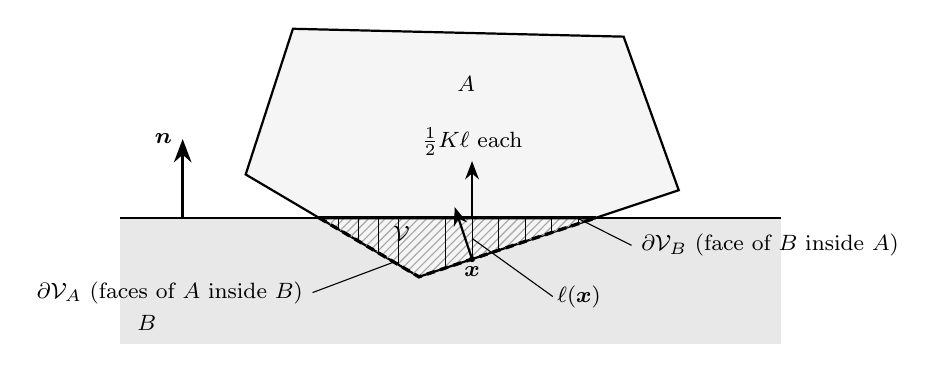
\begin{tikzpicture}[scale=1.0, font=\footnotesize, >=Stealth]
  % Body B (ground with a step, so that the contact is not a single plane)
  \coordinate (b1) at (-4.2,0);
  \coordinate (b2) at (4.2,0);
  \fill[gray!18] (-4.2,-1.6) rectangle (4.2,0);
  \draw[thick] (b1) -- (b2);
  \node[anchor=south west] at (-4.1,-1.55) {$B$};
  % Body A: a wedge-like convex polygon pressed into B, tilted.
  \coordinate (a1) at (-2.6,0.55);
  \coordinate (a2) at (-0.4,-0.75);
  \coordinate (a3) at (2.9,0.35);
  \coordinate (a4) at (2.2,2.3);
  \coordinate (a5) at (-2.0,2.4);
  \fill[gray!8] (a1) -- (a2) -- (a3) -- (a4) -- (a5) -- cycle;
  \draw[thick] (a1) -- (a2) -- (a3) -- (a4) -- (a5) -- cycle;
  \node at (0.2,1.7) {$A$};
  % Intersections of A's lower edges with y = 0.
  \coordinate (p) at ($(a1)!{0.55/1.30}!(a2)$);   % on edge a1-a2 at y=0
  \coordinate (q) at ($(a2)!{0.75/1.10}!(a3)$);   % on edge a2-a3 at y=0
  % Overlap
  \fill[pattern=north east lines, pattern color=gray!70] (p) -- (a2) -- (q) -- cycle;
  \draw[very thick] (p) -- (q);                    % part of dV on B
  \draw[very thick, densely dashed] (p) -- (a2) -- (q);   % part of dV on A
  % Columns along n = +y: from A's faces up to B's face, and from B's face down to A's faces.
  \foreach \t in {0.2,0.4,0.6,0.8} {
    \coordinate (s) at ($(p)!\t!(a2)$);
    \draw[thin] (s) -- (s |- b1);
  }
  \foreach \t in {0.15,0.3,0.45,0.6,0.75,0.9} {
    \coordinate (s) at ($(a2)!\t!(q)$);
    \draw[thin] (s) -- (s |- b1);
  }
  % One column labelled.
  \coordinate (x) at ($(a2)!0.3!(q)$);
  \fill (x) circle (1.1pt) node[below, inner sep=2.5pt] {$\x$};
  \draw[thin] ($(x)!0.5!(x |- b1)$) -- (1.3,-1.0) node[right, inner sep=1.5pt] {$\ell(\x)$};
  % Pair normal.
  \draw[->, very thick] (-3.4,0) -- ++(0,1.0) node[left] {$\n$};
  % Half pressures on both ends of the column.
  \draw[->, thick] (x) -- ++(-0.22,0.66);
  \draw[->, thick] ($(x |- b1)+(0,0.02)$) -- ++(0,0.7) node[above, inner sep=1.5pt] {$\tfrac12 K\ell$ each};
  % Labels
  \node[anchor=west] at (2.3,-0.35) {$\partial\region_B$ (face of $B$ inside $A$)};
  \draw[thin] (2.3,-0.35) -- ($(p)!0.93!(q)$);
  \node[anchor=east] at (-1.75,-0.95) {$\partial\region_A$ (faces of $A$ inside $B$)};
  \draw[thin] (-1.75,-0.95) -- ($(p)!0.75!(a2)$);
  \node at (-0.62,-0.2) {$\region$};
\end{tikzpicture}

\caption{Section of the overlap $\region$ of a body $A$ pressed into a body $B$. The pair
normal $\n$ is the direction of the vector area of $\partial\region_B$ (thick line). Columns run
along $\n$ from the faces of $A$ and along $-\n$ from the faces of $B$; the length $\ell(\x)$ of a
column is the distance to the first face of either body. Each end of a column carries half of
$K\ell$, as a pressure along the normal of its own face}
\label{fig:columns}
\end{figure}

Three constructions make the normal wrench exact for the polyhedra, with no quadrature error
and no dependence on the triangulation; one triangle per flat face is enough. Each polygon of
the contact surface is split into the convex regions where one face ends the column, on which
$\ell$ is affine (Section~S1.6). Where the affine factor $\varphi$ changes sign the region is
cut along $\varphi = 0$ and the tensile side carries no pressure, since there is no adhesion.
On what remains the pressure is the product of two affine functions, whose force and moment
over a triangle have a closed form; each triangle stores the linear pressure $\tilde p$ with
the same force and moment (Section~S1.7), which is the exact pressure whenever $\ell$ or
$\varphi$ is constant on it. Hasegawa and Sato \cite{Hasegawa2004} obtain the exactness of the
elastic term in another way, with a depth that is linear on the triangles of the intersection
polyhedron.

For a flat contact the law reduces to Gonthier's normal wrench: since $\n\cdot\vv$ is constant
along each column and affine in position,
\begin{equation}
  \int K\,\ell\,(1 - h\,\n\cdot\vv)\,\dd A
  = K\!\int_{\region} (1 - h\,\n\cdot\vv)\,\dd V
  = K V \left(1 - h\,\n\cdot\vv(\vect{c})\right),
  \label{eq:reduction}
\end{equation}
and the first moment of the damped pressure is, up to a term of the order of the depth, the
rolling resistance $\vect{M}_r$ of Eq.~\eqref{eq:gonthier-normal}: under a rolling body the
leading half of the patch is loaded more than the trailing half. The rolling resistance is a
property of the foundation with damping, not an addition to it, and the results have to account
for it in the problems whose rigid-body theory has none (Section~\ref{sec:classA}).

\subsection{Coulomb friction in closed form}\label{sec:friction}

Every triangle of the contact surface carries a linear pressure $p$ and slips with the relative
velocity field of the two bodies. The friction traction on $A$ is $-\mu\,p\,\vv_t/|\vv_t|$, with
$\vv_t$ the projection of $\vv$ on the plane of the triangle, and its integral is not a
polynomial: the direction of the slip changes over the triangle. It can nevertheless be done in
closed form, because the slip field of a rigid motion in a plane is a rotation about a point.
Let $\m$ be the unit normal of the triangle, $\x_0$ one of its vertices, $\omega_m = \w\cdot\m$
and $\vv_{t0}$ the tangential velocity at $\x_0$. Then
\begin{equation}
  \vv_t(\x) = \omega_m\,\m\times\rr ,
  \qquad \rr = \x - \q, \qquad \q = \x_0 + \frac{\m\times\vv_{t0}}{\omega_m} ,
  \label{eq:centre}
\end{equation}
where $\q$ is the instantaneous centre of the slip in the plane of the triangle; it need not
lie inside the triangle (Fig.~\ref{fig:slip}). Writing the pressure about the centre,
$p(\x) = p_q + \nabla p\cdot\rr$, with $\sigma = \operatorname{sgn}\omega_m$, the friction force
on $A$ and its moment about $\q$ are
\begin{align}
  \vect{F}_f &= -\mu\,\sigma\,\m\times\int p\,\frac{\rr}{|\rr|}\,\dd A
     = -\mu\,\sigma\,\m\times\left(p_q\,\vect{U} + \tens{W}\,\nabla p\right), \label{eq:friction-force}\\
  \vect{M}_f &= -\mu\,\sigma\int p\,\rr\times\frac{\m\times\rr}{|\rr|}\,\dd A
     = -\mu\,\sigma\left(p_q\,D + \nabla p\cdot\vect{R}\right)\m , \label{eq:friction-moment}
\end{align}
with four \emph{polar moments} of the triangle $T$ about $\q$,
\begin{equation}
  D = \int_T |\rr|\,\dd A, \quad
  \vect{R} = \int_T \rr\,|\rr|\,\dd A, \quad
  \vect{U} = \int_T \frac{\rr}{|\rr|}\,\dd A, \quad
  \tens{W} = \int_T \frac{\rr\,\rr^{\mathsf T}}{|\rr|}\,\dd A .
  \label{eq:moments}
\end{equation}
$D$ and $\vect{U}$ are the moments that Jia \cite{Jia1997} gives for a polygon under uniform
pressure; $\vect{R}$ and $\tens{W}$ are what the linear term of the pressure adds.

\begin{figure}[t]
\centering
% Slip field about the instantaneous centre, and the polar decomposition for one edge.
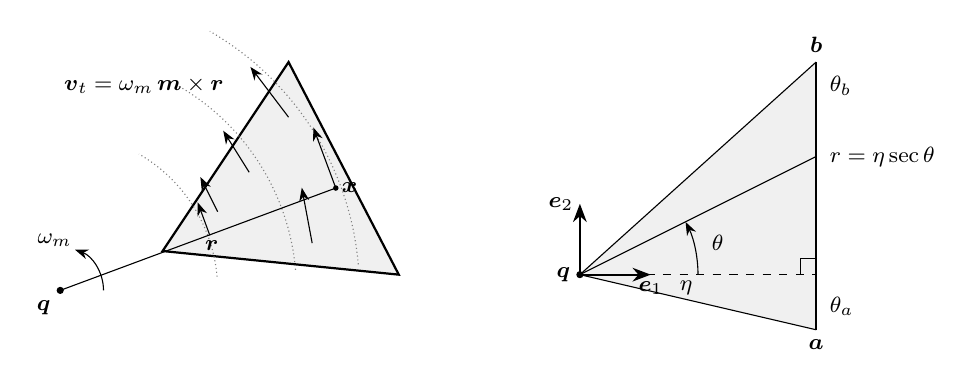
\begin{tikzpicture}[scale=1.0, font=\footnotesize, >=Stealth]
  % ---- Left: slip field -------------------------------------------------------
  \begin{scope}
    \coordinate (q) at (0,0);
    \coordinate (p0) at (1.3,0.5);
    \coordinate (p1) at (4.3,0.2);
    \coordinate (p2) at (2.9,2.9);
    \fill[gray!12] (p0) -- (p1) -- (p2) -- cycle;
    \draw[thick] (p0) -- (p1) -- (p2) -- cycle;
    \fill (q) circle (1.3pt) node[below left] {$\q$};
    % Arcs of the rotation.
    \foreach \rad in {2.0,3.0,3.8} {
      \draw[gray, thin, densely dotted] (5:\rad) arc (5:60:\rad);
    }
    % Slip vectors at sample points: perpendicular to r, length proportional to |r|.
    \foreach \px/\py in {1.9/0.7, 3.2/0.6, 2.4/1.5, 3.5/1.3, 2.9/2.2, 2.0/1.0} {
      \draw[->] (\px,\py) -- ++({-0.22*\py},{0.22*\px});
    }
    \coordinate (x) at (3.5,1.3);
    \draw[thin] (q) -- node[below, pos=0.55, inner sep=2pt] {$\rr$} (x);
    \fill (x) circle (1pt) node[right, inner sep=2pt] {$\x$};
    \node[anchor=east] at (2.2,2.6) {$\vv_t = \omega_m\,\m\times\rr$};
    \draw[->] (0.55,0) arc (0:70:0.55) node[above left, inner sep=1pt] {$\omega_m$};
  \end{scope}
  % ---- Right: polar coordinates for one edge ----------------------------------
  \begin{scope}[xshift=6.6cm]
    \coordinate (q) at (0,0.2);
    \coordinate (a) at (3.0,-0.5);
    \coordinate (b) at (3.0,2.9);
    \coordinate (f) at (3.0,0.2);
    \fill[gray!12] (q) -- (a) -- (b) -- cycle;
    \draw[thick] (a) -- (b);
    \draw (q) -- (a) node[below] {$\vect{a}$};
    \draw (q) -- (b) node[above] {$\vect{b}$};
    \draw[dashed] (q) -- node[below, pos=0.45, inner sep=2pt] {$\eta$} (f);
    \draw (2.8,0.2) -- (2.8,0.4) -- (3.0,0.4);
    \fill (q) circle (1.3pt) node[left] {$\q$};
    \draw[->, thick] (q) -- ++(0.9,0) node[below, inner sep=2pt] {$\vect{e}_1$};
    \draw[->, thick] (q) -- ++(0,0.9) node[left, inner sep=2pt] {$\vect{e}_2$};
    % A ray at angle theta.
    \coordinate (r) at (3.0,1.7);
    \draw[thin] (q) -- (r);
    \draw[->] ($(q)+(1.5,0)$) arc (0:26.5:1.5);
    \node at (1.75,0.6) {$\theta$};
    \node[anchor=west] at (3.05,1.7) {$r = \eta\sec\theta$};
    \node[anchor=west] at (3.05,-0.2) {$\theta_a$};
    \node[anchor=west] at (3.05,2.6) {$\theta_b$};
  \end{scope}
\end{tikzpicture}

\caption{Left: the slip field on a triangle is a rotation about the instantaneous centre $\q$,
with speed $|\omega_m||\rr|$ perpendicular to $\rr$. Right: the triangle is the signed sum of
the three triangles formed by $\q$ and each edge; on the triangle $(\q, \vect{a}, \vect{b})$,
polar coordinates about $\q$ with the angle $\theta$ measured from the perpendicular $\vect{e}_1$
to the edge give $r \le \eta\sec\theta$, with $\eta$ the distance from $\q$ to the line of the edge}
\label{fig:slip}
\end{figure}

The moments are evaluated edge by edge: the triangle is the signed sum of the three triangles
formed by $\q$ and each edge, and in polar coordinates about $\q$ each of them leaves four
elementary integrals whose primitives are an inverse hyperbolic sine and powers of a square
root. Appendix~\ref{app:polar} gives the result, Eq.~\eqref{eq:edge}, and its derivation. The
sign of each contribution comes out of the order of the limits, so no case distinction is
needed for $\q$ inside or outside the triangle, and $\q$ on an edge or at a vertex is not a
singular case. The cost is two square roots and two inverse hyperbolic sines per edge. A
script distributed with the sources re-implements the formulas as printed and compares them
with quadrature that does not use them, for $\q$ outside, inside, on an edge and at a vertex;
they agree to $10^{-14}$ where the integrand is analytic.
% The number of this paragraph is the one paper/checks/check_polar_moments.py prints; it is not a battery result.

The friction is exact for the linear pressure $\tilde p$ of each flat triangle, whatever the
triangulation. It is approximate where $\tilde p$ is not the true pressure (both $\ell$ and
$\varphi$ vary over a triangle), and a uniform-slip formula replaces it when the triangle does
not rotate in its plane or the centre is far (Section~S1.9).

\subsection{Stiction}\label{sec:stiction}

Coulomb friction regularized by velocity alone lets a loaded body creep. Both laws therefore
hold a contact at rest with a bristle: a spring--damper on a tangential deflection $\vect{z}$,
blended with the sliding friction by a weight $s$,
\begin{equation}
\begin{gathered}
  \vect{f} = s\,\vect{f}_\mathrm{stick} + (1-s)\,\vect{f}_\mathrm{slide},
  \qquad \vect{f}_\mathrm{stick} = -k\,\vect{z} - c\,\vv_t, \\
  s = \exp\!\left(-u^2/v_s^2\right),
  \qquad k = \frac{\mu_s\,|\Fn|}{d}, \qquad c = k\,\tau ,
\end{gathered}
  \label{eq:stick}
\end{equation}
and the same for a torsional deflection about $\n$. The speed $u$ is Gonthier's
$v_\mathrm{avg}$ in \law{gonthier} and its counterpart for the pressure distribution in
\law{distributed}. The deflection is the slip of the material point of $A$ at the friction
point, accumulated between evaluations, so that rolling without slipping loads no bristle. The
stiffness is proportional to the load, as in the Dahl and LuGre models and in Gonthier's
bristle \cite{Gonthier2007thesis}: every contact reaches its static limit after the same
displacement $d = 0.1$\,mm, with $\tau = 5$\,ms and $v_s = 24.5$\,mm/s for every contact of
every scenario. The stick force is capped at the static limit, which in \law{distributed} is
the limit surface of the patch approximated by the ellipse of Howe and Cutkosky
\cite{Howe1996}, with the spinning capacity of the pressure distribution from the polar moments
of Eq.~\eqref{eq:friction-moment}, and in \law{gonthier}, as published, a box: force and torque
are limited separately (Section~S1.11).

\subsection{Explicit coupling with the engines and its step limit}\label{sec:coupling}

The contact model is a function: it receives the poses and velocities of the bodies and the
friction state of every pair and returns one wrench per body and the next state. The backends
for Drake 1.58, Project Chrono 10.0 and MuJoCo 4.0 switch the engine's own contact off, apply
the wrenches as external forces and advance (Section~S2.1). In the three the wrench is
\emph{explicit}: computed from the state at the start of the step and held during it, so for
contact the three steppers are the same semi-implicit Euler scheme. Running one law on three
engines therefore checks the implementation on code bases that share nothing, and cannot
separate the error of the law from that of the time discretization, which the step series does
(Section~\ref{sec:convergence}).

An explicit step has a stability limit. A spring $k$ and a damper $c$ acting on an inverse mass
$w$ are stable if and only if $k\,w\,\dt^2 + 2\,c\,w\,\dt < 4$ and $c\,w\,\dt < 2$
(Section~S2.2), and the contributions of the contacts of a body add. For the normal stiffness
of a flat contact of area $A_c$ this is
\begin{equation}
  K A_c\,\dt^2 \sum w < 4 ,
  \label{eq:stability}
\end{equation}
and $< 2$ with the dampers at their bounds: a body of mass $m$ held between two flat contacts,
for which $\sum w = 2/m$, needs $\dt < \sqrt{m/(K A_c)}$. The laws do not change $K$, so
Eq.~\eqref{eq:stability} is the limit of the coupling. The terms proportional to the load (the
stick spring and damper, the normal damper, the slope of the friction across the stick--slip
transition) would impose limits of their own under loads of several times a body's weight; the
laws bound them per unit of load, which changes nothing below a load threshold and, above it,
applies a softer stick, a wider transition and less damping than the parameters say, as
functions of the step (Section~S2.3). An implicit coupling needs the derivatives of the wrench,
which the laws do not provide yet.

\subsection{Baselines from the literature on the same geometry}\label{sec:baselines}

% Describes core/src/pcm.cpp and DistributedParams::friction_quadrature; formulations, sources
% and departures in docs/baselines.md.

Three further methods of the library, run like the two laws with the same $K$, $h$ and $\mu$,
show what the closed-form friction buys and how the closest published law behaves. Two variants
of \law{distributed} replace only the closed form by the quadratures of the literature: the
\emph{vertex rule} of Hasegawa and Sato \cite{Hasegawa2004}, which evaluates the friction at
the three vertices of each triangle and interpolates it linearly, and the \emph{one-point rule},
which applies $-\mu\int p\,\dd A$ along the slip direction at the pressure centroid of each
triangle, as the polygonal contact model, Simbody's elastic foundation and the discrete
hydroelastic model do per element \cite{Hippmann2024,Sherman2011,Masterjohn2022}. When the slip
direction is uniform over a triangle the three rules coincide, so they can differ only where a
contact spins about the normal of its faces. The law \law{pcm} is a per-face elastic foundation
after the polygonal contact model \cite{Hippmann2004,Hippmann2024} and Simbody
\cite{Sherman2011,SimbodyEFF}: every triangle of the surface of one body inside the other is a
spring with one sample of depth, velocity and slip, a normal force
$\tfrac12 K A_T\,x\,(1 + h\,\dot x)$ for a penetration $x$, and a regularized Coulomb friction
without stiction or state, as in its sources. Its elements are the triangles of the exact
contact surface and its depth is measured to the nearest point of the other surface; these and
its other departures from the publications are in Section~S1.13.

\section{The benchmark}\label{sec:benchmark}

% Describes the battery as specified in docs/scenarios.md at the commit of the battery run,
% scripts/bench.sh (run matrix, time limits) and tools/stats.py (statistics). Re-check against
% those files if the battery changes. Table 2 is transcribed from docs/scenarios.md §4: design
% parameters, not results.

The battery is a set of scenarios, each with a set-up, a reference solution and an error
measure, written once against an engine-independent interface and run on every engine with every
contact method.

\subsection{What a reference rests on: classes A, B and C}\label{sec:classes}

Every scenario is classified by what its reference rests on.
\begin{description}
\item[Class A] A rigid-body result that does not depend on the contact model: the acceleration
  of a block on an incline, the time at which a sliding ball starts to roll, the period of a
  ball rolling in a bowl, a wedge that must hold if and only if $\tan\alpha < \mu$. Only these
  scenarios compare a compliant law with a contact model of another kind on equal terms.
\item[Class B] A reference that assumes a pressure distribution: the stop time of a spinning
  disk, ring or cone, the coupled sliding and spinning of a disk, a journal in a bearing without
  clearance. The nominal reference uses the distribution that a rigid body produces on a Winkler
  foundation (uniform for flat faces, a cosine for the journal), so agreement with it is in part
  agreement with the model under test. Other distributions are defensible: uniform wear, the
  rigid punch on an elastic half-space, a line contact. The part of the reference that does not
  depend on the model is the \emph{band} spanned by those distributions: for the disk, the
  friction torque over $\mu N R$ is $2/3$ for uniform pressure, $1/2$ for uniform wear and
  $\pi/4$ for the rigid punch. A method inside the band is not wrong.
\item[Class C] Consistency with the Winkler foundation. The reference contains $K$ or
  integrates the law's own force: the penetrations of a stack, the tilt of an eccentric load,
  the angle at which a tall box tips over a soft support, the rebound of an impact governed by
  the law's own differential equation, the depth reached in a press fit. These scenarios say
  whether a method is a Winkler foundation of stiffness $K$. They do not say whether a method is
  accurate, and they are never used to compare the laws with contact models of another kind.
\end{description}

\subsection{The scenarios}\label{sec:scenarios}

Table~\ref{tab:scenarios} lists the \result{battery/scenarios} scenarios with the quantity that
each one measures; Appendix~\ref{app:scenarios} gives their parameters and references, and the
specification in the repository the dimensions, the mesh criteria and the derivation of each
reference. Four rules hold for all of them. Parameters are fixed before any run, and a scenario
is not changed because a method scores badly on it; the foundations have $K$ between $10^6$ and
$10^8$\,N/m$^3$ and $h = 5$\,s/m. Initial conditions belong to no model: a body that starts in
contact penetrates 1\,\textmu m whatever the method. The reference covers only what it can: the
scenarios of a body rolling on a plane measure what the rigid theory fixes whatever the rolling
resistance of the foundation is (the acceleration at zero speed, the onset of rolling). And the
curved meshes approximate the solid from the inside, with 64 segments per turn in the base
variant; each flat cap of a cylinder, a disk or a frustum is one polygon triangulated as a fan
from one of its rim vertices, and each planar ground is a slab with two triangles per face.

\begin{table}[p]
\caption{The scenarios, by class. $^{2}$: second set (Section~\ref{sec:variants}). For class B
the band of admissible pressure distributions is given as the factor on the nominal stop time}
\label{tab:scenarios}
\footnotesize
\begin{tabular}{@{}lp{0.47\linewidth}p{0.36\linewidth}@{}}
\toprule
Scenario & Set-up & Measured against the reference \\
\midrule
\multicolumn{3}{@{}l}{\emph{Class A: rigid-body references}} \\
\scn{block} & Box sliding down a $30^\circ$ incline & Final velocity \\
\scn{cylinder} & Cylinder rolling down $15^\circ$ from rest & Acceleration at zero speed, slip \\
\scn{sphere} & Sphere rolling down $20^\circ$ from rest & Acceleration at zero speed, slip \\
\scn{push} & Box pushed by a slowly growing force & Onset of sliding, velocity, creep before it \\
\scn{billiard} & Ball launched sliding, without spin & Time and velocity at which rolling starts \\
\scn{vgroove} & Box sliding in a $90^\circ$ groove tilted $30^\circ$ & Final velocity \\
\scn{twoblocks} & Block on a block on a $30^\circ$ incline & Common velocity, no relative slip \\
\scn{bowl} & Ball rolling in a spherical bowl & Period, amplitude (constant) \\
\scn{trough} & Cylinder rolling in a cylindrical trough & Period, amplitude (constant) \\
\scn{journal} & Shaft spinning in a hole with clearance & Stop time, angle of climb \\
\scn{pieces1}, \scn{2}, \scn{8}, \scn{64}$^{2}$ & Sliding and spinning boxes on a table cut into 1, 2, 8 and 64 pieces & Travel, stop time, no drift; same final poses on every cut \\
\scn{wedge}$^{2}$ & Two blocks on a plane tilted slowly; one must hold, one slide & Creep, residual speed, sliding velocity \\
\scn{oblique}$^{2}$ & Spheres hitting a plane obliquely, sliding and sticking & Velocities and spins after the impact \\
\scn{edge}$^{2}$ & Box sliding off the edge of a table & Times at which it has pitched 0.1 and 0.25\,rad \\
\scn{turntable}$^{2}$ & Ball rolling on a free rotating table & Orbit rate, orbit radius (constant) \\
\scn{energy}$^{2}$ & Frictionless, undamped ball sliding in a faceted bowl & Period, drift of the energy \\
\scn{tower}$^{2}$ & Ten stacked blocks, gravity tilted to $5^\circ$ & Nothing moves: creep, residual speed \\
\scn{massratio}$^{2}$ & A 1\,kg block under a 1000\,kg block & Nothing moves: creep, residual speed \\
\midrule
\multicolumn{3}{@{}l}{\emph{Class B: references that assume a pressure distribution}} \\
\scn{disk} & Disk spinning flat on a plane & Stop time (band 0.85--1.33) \\
\scn{contensou} & Disk sliding and spinning & Stop time (band 0.95--1.12) \\
\scn{ring} & Annulus spinning flat & Stop time (band 1--1.02) \\
\scn{bearing} & Shaft spinning in a hole of its own radius & Stop time (band 0.81--1.27) \\
\scn{cone} & Frustum spinning in a conical seat & Stop time (band 1--1.04) \\
\midrule
\multicolumn{3}{@{}l}{\emph{Class C: consistency with the Winkler foundation}} \\
\scn{tip} & Tall box, gravity tilted slowly & Tipping angle on the foundation \\
\scn{drop} & Box dropped flat & Rebound velocity of the law's impact equation \\
\scn{hole} & Cube entering a square hole with interference & Depth at which friction stops it \\
\scn{corner} & Cube pressed into a corner & Penetrations on the three faces \\
\scn{offset} & Plate with an eccentric centre of mass & Tilt at rest \\
\scn{stack} & Three cubes, gravity tilted to $5^\circ$ & Compressions; creep \\
\scn{restitution}$^{2}$ & Spheres hitting a plane at four speeds & Rebounds of the law's impact equation \\
\botrule
\end{tabular}
\end{table}

\subsection{The error of a run}\label{sec:error}

The error of a run is the worst normalized deviation of every quantity that the reference
fixes, and not of the main result alone, so that a box that creeps before the onset of sliding
and then reaches the right velocity is not scored as correct. A value with a non-zero reference
is normalized by that reference, and a quantity that the reference keeps at zero (creep, drift,
relative slip, residual speed) by a length or a speed of the body. A run \emph{holds} when it
finishes with an error below 100\,\%; it is \emph{lost} when the error is larger (bodies thrown
apart or sliding away), and it has \emph{no value} when it diverges, exceeds its time limit or
never produces a quantity of the reference (a body that never stopped or never tipped). The
battery records the size of each term and not its sign, so for class B a run is known to be
inside the band when its error is below the narrow side of the band, outside when it is above
the wide side, and undetermined in between. Errors are not commensurable across scenarios:
methods are compared within a scenario, and summaries across scenarios use counts at fixed
thresholds and ratios of the errors of two methods on the same scenario, never means of errors.

\subsection{Variants, methods and native models}\label{sec:variants}\label{sec:natives}

Every scenario is run in a base variant (64 segments per turn, $\dt = 1$\,ms) and in series:
the step ($\dt = 2$, 0.5, 0.2 and 0.1\,ms), the mesh (32 and 128 segments per turn, for the
scenarios with curved surfaces), the stiffness ($K\times10$ at $\dt = 0.2$\,ms, not for class
C) and eight perturbations of the initial velocities. The matrix is run with the six methods of
the library on each of the three engines (\law{gonthier}, \law{gonthier-thesis},
\law{distributed}, its two friction quadratures and \law{pcm}) and with six native models, each
with a wall-clock limit. Twenty-one scenarios were written while the laws were being developed;
the other twelve, the \emph{second set}, were written with their references before any law was
run on them, and the laws were changed after their first run (Section~\ref{sec:limitations}).

The native models stand for three families, and the results are read by family. \emph{Point
contact}: Drake's compliant point contact, Chrono's penalty model on a collision manifold (SMC)
and MuJoCo's soft constraints with its recommended and with its default parameters; a contact
between two faces is a few points with a stiffness in N/m, so a pressure distribution over the
face is not part of the model. \emph{Complementarity contact}: Chrono NSC, rigid contact with
Coulomb friction, in which $K$ and $h$ do not enter, so class C does not apply to it.
\emph{Pressure-field contact}: Drake hydroelastic, configured with a modulus $E = K H$ so that
the pressure is $K$ times the depth; it is then the same pressure model as the two laws near
the surface, evaluated on tetrahedral fields, and its comparison with \law{distributed} is one
of two discretizations. Each model has one configuration for every scenario, built from the
engine's documentation \cite{DrakeHydroGuide,DrakeHydroParams,DrakePointContact,DrakeFoamBrick,
ChronoCollisions,ChronoSMCSource,ChronoSystem,Barzilai1988,MuJoCoDocs,MuJoCoModeling}; the
configurations are ours and were not reviewed by the developers of the engines, so the main
text draws from the native runs only what follows from a property of the model family, and
Section~S3 gives the configurations and every other result, labelled as results of our
configurations. In the tables the methods are abbreviated Gon (\law{gonthier}), G18
(\law{gonthier-thesis}), Dis (\law{distributed}), Dis-v and Dis-1 (its vertex and one-point
friction rules), PCM, Dr-h and Dr-p (Drake hydroelastic and point), Ch-S and Ch-N (Chrono SMC
and NSC) and Mj-s and Mj-d (MuJoCo soft and default); the methods of the library are shown by
their runs on Chrono.

\section{Results}\label{sec:results}

% Every number, table and figure of this section comes from paper/generated/, which
% tools/paper_results.py writes from results/battery.csv, results/terms.csv, results/stats.json,
% results/ablation_triangulation.csv and paper/provenance.json (see paper/README.md). Predictions
% and the numbers of single diagnostic runs are taken from docs/history.md and
% docs/research/anomalies.md, are worded as such and are marked in comments.

\subsection{The runs, and the same law on three engines}\label{sec:runs}\label{sec:independence}

There are \result{battery/runs} runs: \result{battery/scenarios} scenarios,
\result{battery/methods} combinations of engine and contact method and up to
\result{battery/variants} variants per scenario. Of them, \result{battery/ok} finished with an
error value and \result{battery/failed} did not; the two laws have \result{status/laws/notok}
such run, and Section~S4.1 accounts for each. Errors are in percent of the reference, and the
tables show the base variant.

For \law{gonthier} and \law{distributed}, in the \result{ind/distributed/n} scenarios that
hold, the errors on the three engines differ by at most \result{independence/worst} (in
\result{ind/distributed/worst-scenario}), with a median relative difference of
\result{ind/distributed/median} (Section~S4.2). The three backends pass the same states to the
library and apply its wrenches at the same instant, on code bases that share nothing: this is a
check of the implementation, and the reason why one engine is enough to show a law.

\subsection{Class A: rigid-body references}\label{sec:classA}

Table~\ref{tab:errors-A} gives the errors on the \result{battery/n/A} class A scenarios. Where a
body slides or rolls on one plane (\scn{block}, \scn{cylinder}, \scn{sphere}, \scn{push},
\scn{vgroove}, \scn{twoblocks}, \scn{billiard}) both laws are within 1\,\%, except for the time at which rolling starts in \scn{billiard}
(\result{err/billiard/gonthier} and \result{err/billiard/distributed}), and they hold the
bodies that must be held (\scn{push}, \scn{wedge}, \scn{tower}). A patch model adds nothing
there: a rigid body on one plane is what point and complementarity contact are built for. The methods without a stick state creep long before
the friction limit: \law{gonthier-thesis} and \law{pcm} have \result{err/push/thesis} and
\result{err/push/pcm} in \scn{push}, and \result{err/wedge/thesis} and \result{err/wedge/pcm}
in \scn{wedge}. The larger errors of the two laws have four causes, each of which can be
predicted.

\begin{table}[t]
\caption{Class A: error [\%] of each method, base variant (abbreviations in
Section~\ref{sec:variants}; methods of the library on Chrono). The columns of the native models
are results of our configurations (Section~S3). \textit{nan}, \textit{timeout}: runs without an
error value}
\label{tab:errors-A}
\generatedtable{errors_class_A}
\end{table}

\emph{Rolling resistance of the damped foundation} (\scn{bowl}, \scn{trough}, \scn{turntable}).
In \scn{bowl} and \scn{trough} the period is right (for \law{distributed},
\result{term/bowl/distributed/period} and \result{term/trough/distributed/period}); the error is
the loss of amplitude, which the rigid theory keeps constant: \result{err/bowl/distributed} and
\result{err/trough/distributed}. In \scn{turntable}, whose rigid orbit is a closed circle, the
orbit rate is right (\result{term/turntable/distributed/orbit_rate}) and the orbit spirals
outwards: its radius grows by \result{err/turntable/distributed}. These errors are the rolling
resistance $\vect{M}_r = -K h\,\tens{J}\,\w_t$ of Eq.~\eqref{eq:gonthier-normal}. For the cap of
a sphere of radius $R$ pressed to a depth $\delta$, $\tens{J}$ has the tangential moment
$V R\delta/3$, so the torque is $-(h\,m g R\delta/3)\,\w_t$. In \scn{turntable} the no-slip
equations with that torque give a radius that grows as $\exp(\tfrac{25}{42}\,h g\,\delta\,t/R)$,
that is, by 77\,\% over the run for the static penetration of the scenario, against
\result{err/turntable/distributed} measured; in \scn{bowl} the same torque predicts a loss of
amplitude of 12\,\%, against \result{err/bowl/distributed} measured.
% 77 % and 12 % (0.351 rad left of 0.4): predictions derived in docs/history.md (entries of 2026-11-11), not battery results.
The errors are the model's answer at the $h$ and $K$ of the scenario, not numerical errors: any
damped Winkler foundation has this torque, every Winkler-type method of
Table~\ref{tab:errors-A} shows the loss, and with
$K\times10$ the errors of \law{distributed} fall from \result{err/turntable/distributed/dt0.2}
to \result{err/turntable/distributed/stiff} and from \result{err/bowl/distributed/dt0.2} to
\result{err/bowl/distributed/stiff}.

\emph{Compliance} (\scn{edge}). A rigid block leaves the table when its centre of mass passes
the edge; on a compliant foundation it pitches earlier, and every Winkler-type method does
(\result{err/edge/distributed} for the two laws, \result{err/edge/hydro} for Drake
hydroelastic). With $K\times10$ the error of the laws falls to
\result{err/edge/distributed/stiff}. These four scenarios measure $h$ and $K$ more than the
contact law, and summaries of class A are also given without them (``reduced'' class A).

\emph{The stability bound of the explicit coupling} (\scn{massratio}). The light block between
the heavy one and the ground is held by two contacts, so Eq.~\eqref{eq:stability} requires
$\dt < \sqrt{m/(K A_c)}$, which is 0.25\,ms for the scenario.
% K A_c = 1.6e7 N/m, m = 1 kg: design parameters of the scenario (docs/scenarios.md)
The two laws are lost at 2, 1 and 0.5\,ms and hold from 0.2\,ms, with
\result{err/massratio/distributed/dt0.2} of error at 0.2\,ms and
\result{err/massratio/distributed/dt0.1} at 0.1\,ms, a residual speed that the bounded dampers
remove slowly. A formulation that is implicit in the contact force has no such bound, and
complementarity contact holds the scenario at the base step. The tower of ten blocks is inside the
bound and both laws hold it at the base step (\result{err/tower/distributed}).

\emph{One normal per pair of convex pieces} (\scn{journal}). The error of \law{distributed}
(\result{err/journal/distributed}) is in the angle at which the shaft rides up the hole, and it
does not fall with the mesh (Section~\ref{sec:convergence}).

Two more results concern the laws. On a ground cut into 1, 2, 8 and 64 pieces
\law{distributed} gives the same error (\result{err/pieces64/distributed}); \law{gonthier} is
unaffected up to 8 pieces and turns the spinning box differently on 64
(\result{err/pieces64/gonthier}), and \law{pcm} depends on the cut
(\result{err/pieces64/pcm}). In \scn{oblique} the laws miss the rigid impulse theory by
\result{err/oblique/gonthier} and \result{err/oblique/distributed}.

\emph{Energy} (\scn{energy}). The error is the change of kinetic plus gravitational energy of a
frictionless, undamped ball between the first and the last period. The measure omits the energy
held by the undamped bounce on the contact spring, and sinking to the static penetration alone
moves 2.9\,\% of the energy of the swing, % 2.9 %: m g delta over the swing's energy, docs/research/anomalies.md §2
so it varies irregularly with the step and with the start for every law: over the five steps of
the series between \result{err/energy/gonthier/dt0.2} and \result{err/energy/gonthier/dt2} for
\law{gonthier}, between \result{err/energy/pcm} and \result{err/energy/pcm/dt0.2} for \law{pcm}
and between \result{err/energy/distributed/dt0.5} and \result{err/energy/distributed/dt0.1} for
\law{distributed}. The \result{err/energy/gonthier} of \law{gonthier} in
Table~\ref{tab:errors-A} is one value of that measure and not a steady gain. There is also a
true, smaller effect: Gonthier's normal force $K V\n$ is the gradient of a potential only where
the contact area is a function of the volume alone; with $\nabla V = A_c\n$ its curl is
$-K\,(V/A_c^2)\,\nabla A_c\times\nabla V$, which does not vanish on faceted or decomposed
surfaces. Its size was not separated from the noise of the measure (Section~S4.7).

\subsection{Class B: references that assume a pressure distribution}\label{sec:classB}

Table~\ref{tab:errors-B} gives the errors against the nominal reference and marks the position
of each run against the band of admissible distributions, which is the part of the reference
that does not depend on the Winkler model.

\begin{table}[t]
\caption{Class B: error [\%] against the nominal reference, base variant. Band: admissible
pressure distributions, in percent of the nominal stop time. $^\dagger$: the error exceeds the
wider side of the band, so the run is outside it; $^{*}$: it exceeds the narrower side only, so
its position is undetermined (the sign of the error was not recorded); unmarked errors are
inside. The columns of the native models are results of our configurations (Section~S3)}
\label{tab:errors-B}
\generatedtable{errors_B}
\end{table}

No elastic-foundation method is outside the band in any scenario: \law{distributed},
\law{gonthier}, \law{pcm} and Drake hydroelastic have no run marked as outside
(\law{gonthier-thesis} is the exception among the methods of the library). \law{distributed}
and Drake hydroelastic, the two methods that integrate the foundation over the contact surface,
are known to be inside the band in \result{band/distributed/inside} and
\result{band/hydro/inside} of the five scenarios and are undetermined in the others;
\law{gonthier} and \law{pcm} are inside in fewer. The two also meet the nominal value, within
\result{err/bearing/distributed} and \result{err/cone/hydro}. That agreement is a consistency
result: the nominal value is the model's own distribution, so two independent implementations
of the same pressure model, on different engines and with different discretizations, integrate
it correctly, and nothing follows about whether that pressure is the true one. How far it is
from the pressure of a continuum support is measured, for two of the scenarios, in
Section~\ref{sec:fem}.

\law{gonthier} misses the nominal value by the amount that its lumping predicts:
\result{err/disk/gonthier} in \scn{disk}, where the torque through the radius of gyration is
6\,\% above the exact integral (Section~\ref{sec:gonthier}), and
\result{err/contensou/gonthier} in \scn{contensou}. \law{pcm} has the error of its one-point
friction on the battery's meshes (\result{err/disk/pcm}; Section~\ref{sec:ablation}) and the
smallest error of all methods in \scn{bearing} (\result{err/bearing/pcm}), where its depth
follows the local surface.

A point-contact model does not represent the distribution. A face held by points of its
rim has the friction torque of a ring, $\mu N R$ against $\tfrac23\mu N R$ for the disk, unless
the user supplies a torsional friction coefficient for each geometry; the same holds for
complementarity contact on the same contact points. In the table, each of these models is
outside the band in \result{band/smc/outside} to \result{band/dpoint/outside} of the five
scenarios, and several of their runs scatter over nearby starts or end without a stop time
(Section~S3.4).

% An independent finite-element reference for two class B scenarios (disk, bearing).
% Input by sections/05-results.tex after the class B results. The solver, the cases and the
% numbers of Table~\ref{tab:fem} come from tools/fem (uv run tools/fem/run.py; results/fem/).
% The abstract, Section 7 and Section 8 repeat the 18 % of disk; change them with this file.
\subsection{A finite-element reference for two class B scenarios}\label{sec:fem}

The class B references assume a pressure distribution, and the band lists the alternatives. To
place a continuum in that band we solved, by finite elements, the static frictionless contact of
a linear-elastic support with a rigid body (small strain, quadratic quadrilaterals, unilateral
contact solved exactly by an active set; \code{tools/fem}). For \scn{disk}, an axisymmetric layer
of thickness $H$ bonded to a rigid base under a rigid flat punch of radius $R$; the torque of
sliding everywhere is $f\mu NR$ with $f=\int p\,r\,\dd A/(NR)$. The friction of a spin is
circumferential and, in linear elasticity, uncoupled from the normal problem, so the frictionless
pressure is exact for the spinning punch. For \scn{bearing}, a plane-strain sleeve of wall $t$
bonded to a rigid housing around a rigid journal without clearance, with $E$ such that
$E(1-\nu)/((1+\nu)(1-2\nu)t)$ is the battery's $K$; the torque with the friction circle is
$f\mu Nr/\sqrt{1+\mu^2}$ with $f=\int p\,\dd s/|\int p\,\n\,\dd s|$. There the friction couples
with the normal problem, and the frictionless pressure is its $\mu\to0$ limit. The solver
reproduces the flat punch on a deep layer ($f=\pi/4$ within 0.2\,\%), the Winkler limit of a thin
compressible layer ($f=2/3$) and Hertz line contact (half-width within one node, pressure within
1\,\% of its peak). Over three refinements the ratios of \scn{disk} converge with observed order
2.2 to 2.8 and those of \scn{bearing} change by less than $10^{-4}$; every digit of
Table~\ref{tab:fem} is converged; the pressures are plotted in Section~S4.4. The stop time follows from the scenario's own formula,
$t=I\omega_0/\tau\propto1/f$.

\emph{\scn{disk}.} A thin layer is a Winkler foundation: for $H/R\le0.2$ the pressure is nearly
uniform and $f$ is within 3\,\% of the nominal $2/3$ (below it for $\nu=0.45$, towards the
parabolic pressure of an incompressible thin layer). The shear between neighbouring fibres, which
a Winkler foundation omits, moves the load to the rim as the layer thickens, and the battery's
slab ($H/R=4$) is a half-space: $f$ is $\pi/4$ within 0.3\,\% for both $\nu$. A continuum support
puts \scn{disk} at the rigid-punch end of its band, with a stop time 15\,\% shorter than the
nominal one. No elastic-foundation method models that rim: \law{distributed} and Drake
hydroelastic, which reproduce the uniform pressure of their own model, stop 18\,\% late against
the FE reference, \law{pcm} 29\,\%; \law{gonthier} comes closest (11\,\%) because its lumped
torque is 6\,\% high, an error of the lumping and not a model of the rim. The 18\,\% is therefore a
limit of the Winkler foundation itself on a thick support, shared by its two independent
integrations, and not an error of their discretization; a finer mesh or a smaller step would not
reduce it.

\emph{\scn{bearing}.} For $\nu=0.3$ the continuum sleeve gives the Winkler cosine ($f$ within
0.2\,\% of $4/\pi$, contact over $\pm86^\circ$); a nearly incompressible wall ($\nu=0.45$)
spreads the load beyond the lower half ($\pm94^\circ$) and lies between the cosine and the
$\sqrt{\cos}$ distribution. The two ends of the band, line contact and uniform pressure, are
excluded. Against the FE stop time \law{pcm} and Drake hydroelastic are within 0.7\,\% and
\law{distributed} and \law{gonthier} within 2\,\% at $\nu=0.3$, and all four within 5\,\% at
$\nu=0.45$: the reference does not separate them, since its own dependence on $\nu$ is as large as
their differences, but it confirms that the nominal reference of \scn{bearing} is that of a
continuum and that the large errors of the point-contact models are theirs.

What the FE reference does not settle: it is static, small-strain and frictionless in the normal
problem, and it assumes sliding everywhere; the runs are dynamic and damped. The support's
$\nu$ is not given by the battery, and $E$ follows from $K$ through the thin-layer mapping, which
fixes the sink (the continuum's differs from the Winkler sink by $-5$ to $+22\,\%$) but not $f$.
The battery's ground is defined as a Winkler foundation, so agreement with the nominal reference
remains the right test of whether a method integrates its own model; the FE reference measures
how far that model is from a continuum. \scn{ring} and \scn{contensou}, flat faces on the same
slab, should move towards the rim as \scn{disk} does; they and \scn{cone} were not computed. The
signs in Table~\ref{tab:fem} come from the viewer's export of the committed battery, which
\code{tools/fem/run.py} checks against \code{results/battery.csv}.

% generated by tools/fem: typed from results/fem/fem_reference.csv (converged rows) and
% results/fem/stop_times.csv (engine Drake for the methods of the library; Chrono and MuJoCo
% differ by less than 0.1 %). Rerun tools/fem/run.py and retype if either file changes.
\begin{table}[!tbp]
\caption{Finite-element reference. Top: $f$ of a continuum support against the band (\scn{disk}:
nominal $2/3$, half-space punch $\pi/4\approx0.785$, uniform wear $1/2$; \scn{bearing}: nominal
$4/\pi\approx1.273$, line contact 1, $\sqrt{\cos}$ 1.371, uniform $\pi/2$). Bottom: deviation of
the base-variant stop time [\%] from the nominal reference and from the FE one (\scn{disk}: the
slab with $\nu=0.3$; $\nu=0.45$ moves it by at most 0.1 point)}
\label{tab:fem}
\centering\small
\begin{tabular}{@{}lcccc@{}}
\toprule
\scn{disk}, $f$ & $H/R=0.05$ & $0.2$ & $1$ & $4$ (battery) \\
\midrule
$\nu=0.3$  & 0.671 & 0.685 & 0.750 & 0.784 \\
$\nu=0.45$ & 0.654 & 0.659 & 0.741 & 0.783 \\
\midrule
\scn{bearing}, $f$ & small load & battery load & contact & $E$ [kPa] \\
\midrule
$\nu=0.3$  & 1.272 & 1.276 & $\pm86^\circ$ & 14.9 \\
$\nu=0.45$ & 1.309 & 1.314 & $\pm94^\circ$ & 5.27 \\
\bottomrule
\end{tabular}

\medskip
\begin{tabular}{@{}lrrrrr@{}}
\toprule
& \multicolumn{2}{c}{\scn{disk}} & \multicolumn{3}{c}{\scn{bearing}} \\
\cmidrule(lr){2-3}\cmidrule(l){4-6}
Method & nominal & FE & nominal & FE, $\nu=0.3$ & FE, $\nu=0.45$ \\
\midrule
\law{distributed}  & $+0.1$  & $+17.7$ & $+1.6$  & $+1.8$  & $+4.9$ \\
\law{gonthier}     & $-5.6$  & $+11.0$ & $-1.8$  & $-1.6$  & $+1.4$ \\
\law{pcm}          & $+10.0$ & $+29.3$ & $-0.2$  & $+0.0$  & $+3.1$ \\
Drake hydroelastic & $+0.3$  & $+18.0$ & $+0.5$  & $+0.6$  & $+3.7$ \\
\bottomrule
\end{tabular}
\end{table}


\subsection{Class C: consistency with the Winkler foundation}\label{sec:classC}

Class C asks whether a method is a Winkler foundation of stiffness $K$
(Table~\ref{tab:errors-C}); it does not apply to complementarity contact, which has no
compliance, or to a point contact whose stiffness is not areal. \law{distributed} is within
5\,\% in \result{pass/C/distributed/5} scenarios and \law{gonthier} in
\result{pass/C/gonthier/5}; the largest errors are the depth reached in the press fit
(\scn{hole}: \result{err/hole/gonthier} and \result{err/hole/distributed}). For the two laws
these scenarios are regression tests against the law's own closed-form predictions: the tilt
under an eccentric load, the tipping angle on a soft support and the depth of a press fit all
follow from the pressure over the patch. \law{pcm} and \law{gonthier-thesis} fail the scenarios
in which a body must be held by friction (\scn{tip}, \scn{hole}, \scn{stack}). Drake
hydroelastic, the same pressure model, is within 5\,\% in \result{pass/C/hydro/5}; its errors
in the impact scenarios fall with the step (\scn{drop}: \result{err/drop/hydro} at 1\,ms,
\result{err/drop/hydro/dt0.1} at 0.1\,ms), and three others do not and are unexplained
(Section~S3.5).

\begin{table}[t]
\caption{Class C: error [\%] of the methods that are a Winkler foundation, base variant}
\label{tab:errors-C}
\generatedtable{errors_class_C}
\end{table}

\subsection{The friction quadrature and the triangulation}\label{sec:ablation}

On the meshes of the battery the closed-form friction and the two quadratures of the
literature differ widely on the flat contacts that spin: in \scn{disk},
\result{err/disk/distributed} with the closed form against \result{err/disk/vertex} with the
vertex rule and \result{err/disk/centroid} with one point per triangle, at 128 segments per
turn as at 64 (\result{err/disk/vertex/mesh128} and \result{err/disk/centroid/mesh128}); and
with the ground cut into 64 pieces the error of \scn{pieces} goes from
\result{err/pieces1/vertex} to \result{err/pieces64/vertex} with the vertex rule and to
\result{err/pieces64/centroid} with the one-point rule, while the closed form stays at
\result{err/pieces64/distributed} (Section~S4.5). Where nothing spins about the normal of a
face the three rules agree.

The size of those differences is a property of the battery's meshes. The flat cap of a disk is
triangulated as a fan from a vertex of its rim: long triangles that span the face, none with a
vertex at the centre of rotation, and more segments per turn only add more of them. To separate
the rule from the mesh, the three rules were evaluated, in a re-implementation apart from the
library, on a disk and a ring under a uniform pressure spinning in place, and under a tilted
pressure sliding while spinning about a point at half the radius, for several triangulations of
the same face (Table~\ref{tab:triangulation}, Fig.~\ref{fig:triangulation}). The closed form
gives the same wrench on every triangulation, to round-off (largest difference
\result{tri/closed-spread}). On the fan from the rim the one-point rule loses
\result{tri/disk/spin/rim-fan/64/centroid/moment} of the spin torque and the vertex rule
\result{tri/disk/spin/rim-fan/64/vertex/moment}, at any number of segments: these are the
errors behind the battery's stop times. On a fan from the centre the one-point rule has
\result{tri/disk/spin/centre-fan/64/centroid/moment}, while the vertex rule, which interpolates
unit vectors from a vertex that does not slip, still loses
\result{tri/disk/spin/centre-fan/64/vertex/moment}; when the face also slides the centre fan
is no longer a lucky mesh for the one-point rule
(\result{tri/disk/slide+spin/centre-fan/64/centroid/force} of the load in the force). On
well-shaped triangles both rules converge at second order: with
\result{tri/disk/spin/hex/4/centroid/triangles} nearly equilateral triangles the errors are
\result{tri/disk/spin/hex/4/centroid/moment} and \result{tri/disk/spin/hex/4/vertex/moment},
and with \result{tri/disk/spin/hex/16/centroid/triangles},
\result{tri/disk/spin/hex/16/centroid/moment} and \result{tri/disk/spin/hex/16/vertex/moment}.

So the closed form is not more accurate than a well-used quadrature: on a face meshed with a
few hundred well-shaped triangles a one-point rule is within a few tenths of a percent, the
level of the other errors of the battery, and Drake hydroelastic, which uses one point per
polygon of a refined contact surface, has \result{err/disk/hydro} in \scn{disk}. What the
closed form gives is independence: the friction wrench of a flat face does not depend on how
the face is triangulated or on how the bodies are cut into pieces, so a flat face needs no mesh
of its own. A quadrature needs the face remeshed, and its error then depends on the quality of
that mesh.

\begin{table}[t]
\caption{The friction quadratures on one flat face, apart from the battery: error [\%] of the
friction torque of a face spinning in place under uniform pressure, and of the torque and the
force (the latter over $\mu$ times the load) of a face sliding and spinning under a tilted
pressure, against the closed form, which is the same on every triangulation. Negative: too
little torque}
\label{tab:triangulation}
\generatedtable{triangulation}
\end{table}

\begin{figure}[t]
\centering
\generatedfigure[width=0.9\linewidth]{ablation_triangulation}
\caption{Error of the spin torque of a disk under uniform pressure with the one-point rule and
with the vertex rule, against the number of triangles of the face, for five families of
triangulations. The closed form has no error on any of them}
\label{fig:triangulation}
\end{figure}

\subsection{Convergence with the step and the mesh}\label{sec:convergence}

\emph{Step.} The step series of the two laws are mostly flat (a slope of the logarithm of the
error within $\pm0.2$, or every error below $2\times10^{-3}$): \result{convn/dt/distributed/flat}
of \result{convn/dt/distributed/n} for \law{distributed} and \result{convn/dt/gonthier/flat} for
\law{gonthier} (Section~S4.6). Their error at 1\,ms is then mostly not an error of the time
integration but the error of the model against the reference, or of the mesh. Where it is a
step error it falls roughly in proportion to the step (\scn{drop}, \scn{tower}), and
\scn{massratio} shows the stability bound (Section~\ref{sec:classA}).

\emph{Mesh.} The errors of \law{distributed} fall with the number of segments in
\result{convn/mesh/distributed/converging} of the \result{convn/mesh/distributed/n} scenarios
with curved surfaces. Two series that do not converge matter. \scn{journal} is flat
(\result{err/journal/distributed/mesh32}, \result{err/journal/distributed} and
\result{err/journal/distributed/mesh128} at 32, 64 and 128 segments), while \law{pcm} converges
on it (\result{err/journal/pcm/mesh128} at 128): the geometry of \law{distributed} is exact for
the polyhedra, but with one normal per pair of pieces its answer for a curved conforming
contact does not converge to that of the curved bodies. \scn{cone} is not monotone
(\result{err/cone/distributed/mesh32}, \result{err/cone/distributed},
\result{err/cone/distributed/mesh128}), at errors below 1\,\%. In \scn{bearing} the error of
\law{distributed} falls from \result{err/bearing/distributed/mesh32} to
\result{err/bearing/distributed/mesh128}, and that of Drake hydroelastic from
\result{err/bearing/hydro/mesh32} to \result{err/bearing/hydro/mesh128}: a contact surface
without a representative normal converges faster and further on curved conforming contact. The
series have three points, so no order is quoted.

\subsection{A stiffer foundation: friction-induced flutter}\label{sec:stiffness}

The stiffness series has two points, $K$ and $10K$, both at 0.2\,ms: enough to see a direction
and not a limit (Section~S4.7). On class A the error of \law{distributed} falls by more than a
tenth in \result{stiffn/distributed/better} of \result{stiffn/distributed/n} scenarios, among
them those whose error was attributed above to the compliance or to the damping of the
foundation, and
rises in \result{stiffn/distributed/worse} (\scn{cylinder}, and \scn{massratio}, which is
further beyond the stability bound). On class B the stiffer foundation makes the errors of the
two laws larger in \result{stiffn/distributed/worse/B} of the five scenarios: \scn{disk} from
\result{err/disk/distributed/dt0.2} to \result{err/disk/distributed/stiff}, \scn{cone} from
\result{err/cone/distributed/dt0.2} to \result{err/cone/distributed/stiff}, \scn{bearing} from
\result{err/bearing/distributed/dt0.2} to \result{err/bearing/distributed/stiff}.

On the flat \scn{disk} the cause is not the explicit coupling: in diagnostic runs the error at
$10K$ was the same at steps from 1 to 0.05\,ms.
% Diagnostic single runs on Chrono, docs/research/anomalies.md §1: 18.1 % at 0.2 ms, 17.7 % at 0.05 ms; tilt 1.8e-5 rad at K, 1.2e-3 rad at 10 K; growth 6.6 and 32 1/s measured, 6.3 and 31 predicted.
It is a self-excited wobble of the model. A tilt $\vect{\theta}$ of the spinning disk shifts
the pressure, so the friction of the heavier side no longer cancels that of the lighter one: a
net friction force of magnitude $\mu K\,(\pi R^3/3)\,\theta$ appears, and it acts at the
contact, half the thickness $H$ of the disk below the centre of mass. Its moment,
$N_c = \mu K\,(\pi R^3/3)\,(H/2)$ per unit of tilt, turns the tilt instead of restoring it (a
circulatory term), and the whirl grows when
\begin{equation}
  \mu K\,\frac{\pi R^3}{3}\,\frac{H}{2} \;>\; c_\theta\,\omega_\theta ,
  \qquad c_\theta = \frac{h\,m g R^2}{4}, \qquad \omega_\theta = \sqrt{\frac{K I_A}{I_t}} ,
  \label{eq:flutter}
\end{equation}
with $c_\theta$ the rocking damping of the foundation under the weight $m g$,
$I_A = \pi R^4/4$ the second moment of the face and $I_t$ the transverse moment of inertia of
the disk, at the rate $(N_c/\omega_\theta - c_\theta)/(2 I_t)$. For the disk of the scenario
the threshold is $K = 1.9\times10^6$\,N/m$^3$, about twice the scenario's stiffness: at $K$ the
wobble decays, at $3K$ the condition predicts a growth of 6\,s$^{-1}$ and the diagnostic run
showed 6.6, and at $10K$ it predicts 31\,s$^{-1}$ against 32 measured. The tilt saturates at
$1.2\times10^{-3}$\,rad; the disk then rides on its rim, where the friction torque tends to
$\mu N R$, and stops early. The left side of Eq.~\eqref{eq:flutter} grows with $K$ and the
right side with $\sqrt{K}$: a foundation made stiffer at the same $h$ is less damped in
rocking. In general the condition is $\mu K S_\rho\,z_c > c_\theta\,\omega_\theta$, with
$S_\rho$ the first radial moment of the patch and $z_c$ the height of the centre of mass.
Eq.~\eqref{eq:flutter} is therefore a limit of validity of the damped Winkler law with sliding
friction under a body whose centre of mass is above the contact, and not a defect of an
implementation: the linear model reproduces the growth rates of both laws. On the curved seats
(\scn{cone}, \scn{bearing}) every Winkler-type method degrades at $10K$, Drake hydroelastic
included (\result{err/cone/hydro/dt0.2} to \result{err/cone/hydro/stiff}); there the same
self-excited motion and the sag of the facets, which is no longer small against a penetration
ten times smaller, act together and were not separated.

\subsection{Cost}\label{sec:cost}

% The cost numbers are generated from results/timing.csv (scripts/bench.sh --timing on an idle
% machine); without that file the generator falls back to the accuracy pass and labels it.

Costs are wall-clock time over simulated time from \result{cost/source}: every scenario in the
base variant, one run at a time, the median of \result{battery/timing-repeats} repeats, on an
\result{battery/timing-machine} processor (Section~S4.8). \law{gonthier} runs at a median of
\result{cost/gonthier/median} of real time and never above \result{cost/gonthier/max}.
\law{distributed} has a median of \result{cost/distributed/median} and is slower than real time
in \result{cost/distributed/slow} scenarios, the two with spheres hitting a plane, up to
\result{cost/distributed/max}; its cost grows with the number of faces in contact. \law{pcm}
has a median of \result{cost/pcm/median}. The point-contact and complementarity models, as
configured, have medians between \result{cost/mjdefault/median} and
\result{cost/dpoint/median}. Drake hydroelastic computes a contact surface between tetrahedral
pressure fields wherever the ground is not a plane, and solves one constraint per polygon of
that surface; as configured here and at the step of the battery, it has a median of
\result{cost/hydro/median}, is slower than real time in \result{cost/hydro/slow} of the
\result{cost/hydro/n} scenarios that it finished, up to \result{cost/hydro/max} times, and did
not finish \scn{tower} within the limit.

\subsection{Paired comparisons}\label{sec:ratios}

Across scenarios, two methods are compared by the geometric mean of the ratio of their errors
on the same scenarios, with errors capped at \result{rules/cap}, runs without a value counted
at the cap, a bootstrap interval and Holm's correction over a family of \result{primary/n}
primary comparisons: \law{distributed} against \law{gonthier}, and each of the two against one
native model per engine, on class A and on classes A and B (Table~\ref{tab:primary};
Section~S5 has the rules, the sensitivity analyses and the exploratory pairs). Only
\result{primary/significant} of the \result{primary/n} survive the correction, both on classes
A and B together: \law{distributed} has about half the error of \law{gonthier}
(\result{robust/distributed-vs-gonthier/A+B/full}, adjusted $p = $
\result{robust/distributed-vs-gonthier/A+B/holm}) and about a quarter of that of Chrono SMC
(\result{robust/distributed-vs-smc/A+B/full}), the latter narrowly (adjusted $p = $
\result{robust/distributed-vs-smc/A+B/holm}). On class A alone no difference is significant:
the ratios of the laws to the native models are below 1 with intervals that reach above it.
Within 5\,\% of the reference, \law{distributed} solves \result{pass/A/distributed/5} class A
scenarios and \result{pass/B/distributed/5} of class B, and \law{gonthier}
\result{pass/A/gonthier/5} and \result{pass/B/gonthier/5}. The scenarios are few, hand-picked
and correlated, so these figures describe this battery and are not an estimate for other
problems.

\begin{table}[t]
\caption{The primary comparisons: geometric mean of the ratio of the errors of two methods on
the same scenarios (base variant; a law against a native model on that model's engine), with
its 95\,\% bootstrap interval and the Holm-adjusted $p$ over the \result{primary/n}
comparisons. Bold: adjusted $p$ below 0.05}
\label{tab:primary}
\generatedtable{primary_compact}
\end{table}

\section{Discussion}\label{sec:discussion}

% Every statement about results refers to Section 5 and uses its generated numbers. Statements
% about native models are limited to properties of the model family; what the runs of our
% configurations show beyond that is in Section S3.

\paragraph{What a patch model is for.} The answer of a scenario depends on the model of the
patch exactly where it depends on how the pressure is distributed: the friction torque of a
spinning face, the tilt of an eccentric load, the angle at which a body tips over a soft
support, the force that holds a press fit. A point contact represents a face by a few points
with a stiffness in N/m; it gives a disk the friction torque of a ring unless the user supplies
a torsional coefficient per geometry, and it has no areal stiffness against which class C could
be asked. Complementarity contact has no compliance at all, so the same questions do not apply
to it, and it is the natural choice where rigidity is the right model: a body sliding or
rolling on one plane, a body held by friction, stiff contacts on light bodies. On those
problems a patch model adds nothing, and the two laws pay for their foundation with the rolling
resistance of its damping, with its compliance and with the step bound of their explicit
coupling. Table~\ref{tab:decision} sets the situations against the model property that each one
needs.

\begin{table}[t]
\caption{Which property of a contact model each situation needs, as far as classes A and B of
the battery show}
\label{tab:decision}
\footnotesize
\begin{tabular}{@{}p{0.30\linewidth}p{0.33\linewidth}p{0.31\linewidth}@{}}
\toprule
Situation & What it needs & Evidence \\
\midrule
A rigid body sliding or rolling on one plane; sphere and cylinder contacts &
  Nothing beyond point or complementarity contact &
  Both laws within 1\,\% in \result{within/oneplane/distributed+gonthier/1} such scenarios
  (Table~\ref{tab:errors-A}); no gain from the patch \\
A flat face that spins, or slides and spins &
  A pressure distributed over the face: \law{distributed} or a pressure field; \law{gonthier}
  where its lumping error is acceptable &
  \scn{disk}: \result{err/disk/distributed}; \law{gonthier} \result{err/disk/gonthier};
  the rim torque of point contact (Section~\ref{sec:classB}) \\
Curved conforming contact (a journal, a conical seat) &
  Local normals: a per-face foundation or a pressure field. A finer mesh is not a remedy for
  \law{distributed} &
  \scn{journal}: \law{distributed} \result{err/journal/distributed/mesh32},
  \result{err/journal/distributed}, \result{err/journal/distributed/mesh128} at 32, 64 and 128
  segments; \law{pcm} \result{err/journal/pcm/mesh128} at 128 \\
Bodies or grounds cut into convex pieces &
  A wrench independent of the cut: \law{distributed} &
  \scn{pieces64}: \result{err/pieces64/distributed}; \law{gonthier}
  \result{err/pieces64/gonthier}, \law{pcm} \result{err/pieces64/pcm} \\
A body held by friction near its limit &
  A stick state, or a complementarity formulation &
  \scn{push}, \scn{wedge}: the laws below 1\,\%; \law{pcm} \result{err/push/pcm} and
  \result{err/wedge/pcm} \\
Stiff contacts on light bodies, large mass ratios &
  A formulation implicit in the contact force; not the explicit laws beyond
  Eq.~\eqref{eq:stability} &
  \scn{massratio}: the laws lost at 0.5\,ms and above, held from 0.2\,ms \\
Long rolling &
  No damping torque in the patch: rigid contact, or the laws with little damping or a stiff
  foundation &
  \scn{turntable}: \result{err/turntable/distributed};
  \result{err/turntable/distributed/stiff} with $K\times10$ \\
Only surface meshes are available &
  \law{gonthier} (any closed mesh) or \law{distributed} (convex pieces) &
  No volume mesh or pressure field is needed \\
\botrule
\end{tabular}
\end{table}

\paragraph{Lumped, distributed and per-face foundations.} The three are the same normal law.
\law{gonthier} lumps it, which is exact for a flat patch in the normal wrench and costs
\result{err/disk/gonthier} to \result{err/contensou/gonthier} where a face spins. \law{distributed} integrates it, which removes
that error and makes the result independent of the triangulation and of the cut, at a higher cost (medians of
\result{cost/gonthier/median} and \result{cost/distributed/median} of real time). \law{pcm} samples it once per element: what separates it from
\law{distributed} is the friction on coarse flat faces, which a finer mesh would repair, and
the lack of a stick state, which it would not. On curved conforming contact \law{pcm} is the
better of the two, because its depth follows the local normal: exact integration on each face
with a depth measured locally is the pressure field of hydroelastic contact reached from the
other side.

\paragraph{Against pressure-field contact.} With $E = K H$, hydroelastic contact is the same
pressure model as \law{distributed} near the surface, and the comparison is one of
discretizations. \law{distributed} takes surface meshes, needs convex pieces, clips the overlap
exactly and integrates pressure and friction on it in closed form, so that one triangle per
flat face is enough; its contact has one normal per pair of pieces and its coupling is
explicit. Hydroelastic contact needs a pressure field in every compliant body and has no
contact between two rigid geometries; its contact surface is curved, with no representative
normal, so it converges on curved conforming contact where \law{distributed} does not, and its
solver is implicit, so it has no step bound of the kind of Eq.~\eqref{eq:stability}; it pays
for the contact surface between tetrahedral fields and for one constraint per polygon. A user
who needs non-convex geometry, stiff contact or large steps is better served by it; a user who
has surface meshes, moderate stiffness and flat patches that spin, on convex or decomposed
bodies, obtains the same pressure model from \law{distributed}.

\paragraph{What the closed-form friction gives.} Independence of the triangulation and of the
decomposition, exactly and at no cost in mesh (Section~\ref{sec:ablation}). It removes a
requirement on the mesh and is not a gain in accuracy over a well-used quadrature. It is the
only element of \law{distributed} that we claim as new, and it is a direct extension of the
uniform-pressure result of Jia \cite{Jia1997} with the same primitives.

\section{Limitations and threats to validity}\label{sec:limitations}

% The one place where the caveats of the paper are stated. Other sections refer here.

% The finite-element reference (Section 5.4, sections/fem-reference.tex) covers disk and bearing
% only; widen this paragraph if another external reference is added.
\paragraph{One finite-element reference, no experimental one.} Every reference of the battery
is analytic. Class A references are exact for rigid bodies; class B references assume a
pressure distribution; class C references are the foundation's own. For two class B scenarios,
\scn{disk} and \scn{bearing}, Section~\ref{sec:fem} places a linear-elastic continuum in the
band. It settles where a continuum support falls there (on the Winkler cosine for the thin
sleeve, at the rigid-punch end for the battery's thick slab) and that on the thick slab the
methods that integrate the foundation correctly are off by the distance between a Winkler
foundation and a continuum, which no discretization removes. It does not settle more. It is a
static, small-strain solution of the frictionless normal problem, exact for the spinning punch
and the $\mu\to0$ limit for the sleeve, and it assumes sliding everywhere, while the runs are
dynamic, damped and pass through stick; the support's Poisson ratio is not given by the
battery, and $E$ follows from $K$ through the thin-layer mapping. It covers two scenarios:
\scn{ring}, \scn{contensou} and \scn{cone} were not computed, and no class A or C scenario,
impact, rolling resistance or flutter has a continuum reference. Apart from the thin layers of
Section~\ref{sec:fem}, where a continuum behaves as one, nothing in this paper shows that a
Winkler foundation of stiffness $K$ describes a physical contact, and no measurement was used. Conformal cylindrical contact has finite-element and analytic references in the
literature on clearance joints \cite{Liu2007,Pereira2011,Pereira2015}, and patch friction has
experimental ones \cite{Kudra2015}; we cite those works for what their titles and abstracts
state and used none of their reference solutions.

\paragraph{A regime chosen for the laws.} The stiffness of every scenario was chosen so that
the explicit coupling is stable at the base step of 1\,ms, with two exceptions written to show
the limit (\scn{tower}, \scn{massratio}). The foundations are therefore soft, $10^6$ to
$10^8$\,N/m$^3$, orders of magnitude below engineering materials over a layer of millimetres,
where the laws would need a step proportional to $K^{-1/2}$ and solvers implicit in the contact
would not; one decade of stiffness was explored, at one step, and the rigid limit of class A
was not tested. The damping factor $h = 5$\,s/m has no physical justification and was not tied
to a coefficient of restitution; with $K$ it sets the errors of \scn{bowl}, \scn{trough},
\scn{turntable} and \scn{edge}. The stiction constants $d$ and $\tau$ were not swept. The
battery did not record in which runs the step bounds of Section~\ref{sec:coupling} were active;
from the loads, they are in \scn{tower}, \scn{massratio} and \scn{stack} at the base step and
not where one body rests under its own weight. Where they act, what is benchmarked is the law
regularized by the step, and a flat step series is evidence about the law as given only where
they do not.

\paragraph{Few, hand-picked scenarios that the laws have seen.} The
\result{battery/scenarios} scenarios are not a sample of the problems that a user will meet;
several test the same mechanism, and class B has \result{battery/n/B}. The laws were developed
on \result{battery/dev} of them and changed in response; the other \result{battery/heldout},
the second set, were written before any law was run on them, but three changes to the laws were
adopted after their first run (Section~S4.3), so no part of the battery is an out-of-sample
test of the two laws. Every change was general (no scenario has a constant of its own). The
ratios, intervals and $p$-values of Section~\ref{sec:ratios} are therefore descriptive: the
bootstrap treats as exchangeable units that are not, and the family of primary comparisons and
the rules for capped and failed runs were fixed after the data had been seen (Section~S5). The
battery records the class B errors without sign (Table~\ref{tab:fem} signs those of \scn{disk}
and \scn{bearing} from their stop times). The findings that we expect to survive another
battery are those tied to a mechanism, not the counts.

\paragraph{The native configurations and the baselines are ours.} No configuration of a native
model was reviewed by the developers of its engine; they were built from the documentation,
revised after first results on the development scenarios, and contain asymmetries (Section~S3).
The main text therefore claims of the native models only what follows from their model family.
Their other results, several of them unexplained and several scattered over nearby starts, are
in Section~S3 as results of our configurations and should not be read as the performance of
those engines in expert hands. The vertex rule follows our reading of Hasegawa and Sato
\cite{Hasegawa2004}; the paper was not accessible to us again, so the rule was not re-checked
against its equations. \law{pcm} departs from its publications (Section~S1.13), and the
published models on their own meshes were not run. The statements of
Section~\ref{sec:related} about the models of Hasegawa and Fujii, Luo and Nahon, and Wakisaka
and Sugihara rest on the classification of Elandt et al.~\cite{Elandt2019}, not on the primary
sources.

\paragraph{Limits of validity of the laws.} (i) \emph{Explicit coupling}: the normal stiffness
is bounded by Eq.~\eqref{eq:stability}, and above a load threshold the step bounds apply a
softer stick, a wider stick--slip transition and less damping than the parameters say; the
remedy is an implicit coupling with the Jacobians of the wrench. (ii) \emph{Friction-induced
flutter}: beyond Eq.~\eqref{eq:flutter} a sliding face under a body with a raised centre of
mass is unstable in rocking; the ratio of the two sides grows as $\mu\,z_c\sqrt{K}/h$, the
class B scenarios are below the limit at their $K$ and above it at $10K$, and a damping stated
as a time constant, which would reverse that dependence, would change the published law and
every result and was not tried. (iii) \emph{One normal per pair of convex pieces}
\cite{Elandt2019}: non-convex bodies must be decomposed exactly, curved conforming contacts are
represented facet by facet, and \scn{journal} does not converge. (iv) \emph{Energy}: Gonthier's
normal force is not conservative on faceted or decomposed geometry, and the elastic force of
\law{distributed} is not where the pair normal turns with the overlap. (v) \emph{What ``exact''
covers}: the geometry and the normal wrench, for the polyhedra given and not for the curved
bodies that they approximate; the friction is exact for a linear pressure on each flat triangle
and approximate elsewhere, and the stiction is a lumped regularization with two constants that
are not material properties (Sections~S1.8, S1.9 and~S1.11).

\paragraph{Unexplained observations.} \law{pcm}, whose normal law, damping and friction lever
are nominally those of the two laws, did not flutter on the disk up to $100K$. The value of the
energy measure of \law{gonthier} at the base step differs from that of a single run made when
the scenario was written, and the change that moved it was not identified. How much of the
growth of the errors of \scn{cone} and \scn{bearing} at $10K$ is flutter and how much the sag
of the facets was not separated. Section~S5.5 lists the runs that would settle these and the
other open points.

\paragraph{Timings.} The costs are those of one processor, one thread configuration and one
step size; the two friction quadratures were not timed, Chrono SMC is sub-stepped by its
backend, and the native models were run at the step of the battery, not at the larger steps
that implicit solvers allow.

\section{Conclusions}\label{sec:conclusions}

We have presented a battery of \result{battery/scenarios} conforming- and patch-contact
problems with analytic references, classified by what each reference assumes, and run on it two
elastic-foundation laws evaluated on exact mesh intersections, two baselines from the
literature on the same geometry and six native contact models of Drake, Chrono and MuJoCo. The
battery, with its classes, its band of admissible pressure distributions, its error terms and
its rules, is the reusable product of the work; the laws are an open, engine-independent
implementation of known models. The findings are these.
\begin{enumerate}
\item Where the answer depends on the pressure distribution, no elastic-foundation method is
  outside the band of admissible distributions; \law{distributed} and Drake hydroelastic, two
  discretizations of the same pressure model, agree with the model's own distribution within
  \result{err/bearing/distributed} and \result{err/cone/hydro}, which is consistency and not
  validation. A finite-element solution shows where in the band a continuum support falls
  (Section~\ref{sec:fem}): on the Winkler cosine for the thin sleeve of \scn{bearing}, where the
  four foundation methods are within 5\,\% of it and it cannot rank them, and at the rigid-punch
  end for the thick slab of \scn{disk}, against which \law{distributed} and Drake hydroelastic
  stop 18\,\% late. That is a limit of the Winkler foundation itself on a thick support, not of
  the discretization. A point contact gives a face the friction torque of its rim, and Gonthier's
  lumping costs the 6\,\% that its radius of gyration predicts.
\item The failures of the two laws follow from their model or from their coupling, with
  predictions that the runs match: the rolling resistance of the damped foundation makes a
  rolling orbit grow by \result{err/turntable/distributed} against 77\,\% predicted; a spinning
  disk on a foundation ten times stiffer flutters at the threshold and with the growth rates of
  a linear model, Eq.~\eqref{eq:flutter}; the explicit coupling loses a light body between
  stiff contacts above the step of Eq.~\eqref{eq:stability} and holds it below; a compliant
  foundation lets a block pitch over an edge early. One normal per pair of convex pieces stops
  the convergence of \law{distributed} on a journal in a hole with clearance.
\item The closed-form Coulomb friction of a linear pressure on a triangle makes the friction
  wrench of a flat face independent of its triangulation and of the decomposition of the
  bodies. One-point and vertex quadratures lose \result{tri/disk/spin/rim-fan/64/centroid/moment}
  and \result{tri/disk/spin/rim-fan/64/vertex/moment} of the spin torque of a disk triangulated
  as a fan from its rim, whatever the number of segments, and converge at second order on
  well-shaped meshes. The gain is a mesh that is not needed, not accuracy that a quadrature
  cannot reach.
\item Each law gives the same errors on three engines (within \result{independence/worst}
  wherever a run holds), and its step series are mostly flat, so the reported errors are
  mostly those of the model and the mesh. Gonthier's friction as published, with the bristle on
  the material slip, holds the bodies that the variant of the 2018 thesis lets creep.
\item Of \result{primary/n} paired comparisons of errors, \result{primary/significant} survive
  a correction for multiplicity: \law{distributed} has about half the error of \law{gonthier}
  on classes A and B, and about a quarter of that of Chrono SMC, the latter narrowly. On the
  rigid-body references alone nothing separates the laws from the native models.
\end{enumerate}

Two things would change the weight of these conclusions. An implicit coupling, with the
Jacobians of the contact wrench, would remove the step limit that is the main practical
disadvantage of the laws. And an experimental reference, with finite-element ones for the
other scenarios of class B and for the dynamics of the runs, would turn consistency with an
assumed pressure into validation; the static one of Section~\ref{sec:fem} covers two scenarios
(Section~\ref{sec:limitations}).


\backmatter
% Back matter. The statements are factual records of how the work was produced.

\section*{Declarations}

\bmhead{Use of generative AI}
This work was carried out by a generative AI system, listed as first author, under human
direction, and we describe the division of work in full. The software
described in this paper (the engine-independent library, the three engine backends, the
scenarios, the baselines and the tools), the design of the benchmark, the analysis of its
results and the draft of this manuscript were produced with Claude (Anthropic), used through
its coding agent Claude Code, under the direction of the second author. The work, from 10 to 12 November 2026, was carried out mostly by the model
Claude Fable~5.2, which also directed further instances of itself, of Claude Opus~5.5 (an
independent audit of the code and referee reports) and of Claude Sonnet~5.5 (auxiliary tasks:
scripts, packaging, the viewer and the site). The
starting point was the second author's 2018 thesis \cite{Vilela2018} and its code. The second author set the
questions, decided the scope, approved the changes to the contact laws and the rules of the
benchmark. Under that direction the system reviewed the literature and
proposed the framing of the paper as a benchmark; designed and implemented the laws' evaluation,
including the derivation and the numerical check of the formulas of Section~\ref{sec:friction};
audited the first version of the benchmark and redesigned it, including the classification of
the references and the second set of scenarios; configured the native models from the engines'
documentation; ran the battery; wrote the scripts that compute the statistics and generate
every number, table and figure of the paper from the result files; drafted the text; and, in a
further session, wrote a referee's report on the manuscript and revised the analysis and the
text in response to it (12 November 2026). The
schematic figures are diagrams drawn by the system from the geometry of the paper and the plots are generated
from the data; there are no generated images. Every reference in the bibliography was checked
against the publisher's or registry's record, and the repository records which sources were
read in full. The first author is an AI system and cannot be held accountable; the second author
directed the work and is the person to whom questions about it should be addressed.

\bmhead{Funding}
No funding was received for this work.

\bmhead{Competing interests}
The second author has no competing interests to declare; the first author is a commercial AI
system developed by Anthropic.

\bmhead{Data and code availability}
The library, the three engine backends, the scenarios with their references, the mesh generator,
the scripts that run the battery and compute its statistics, and the sources of this paper with
the scripts that generate its numbers, tables and figures and check its derivations and
references are open source under the BSD 3-Clause licence at
\code{https://github.com/dvilelaf/volumetric-contact}. The
build runs in a container with pinned versions of Drake, Project Chrono and MuJoCo. The results
of the battery reported here (\code{battery.csv}, with checksum \result{battery/sha256};
\code{terms.csv}; \code{stats.json}) are part of the repository, one command regenerates from
them every number, table and figure of the paper, and the trajectories of the runs can be
replayed in a viewer published with it. The main matrix was run on \result{battery/date} with
the code of commit \result{battery/commit}; the friction quadratures and \law{pcm} were added
at commit \result{battery/commit-baselines}, after \result{battery/spot-runs} runs spread over
the scenarios reproduced the main matrix (largest relative difference
\result{battery/spot-diff}); the timings are those of commit \result{battery/timing-commit} on
\result{battery/timing-date}. The derivations of the predictions quoted in the text and the
single diagnostic runs behind them are recorded in the history of the repository.

\bmhead{Author contributions}
Claude Fable~5.2: methodology, software, validation, formal analysis, investigation, data
curation, visualization, writing (original draft, review and editing). David Vilela:
conceptualization, supervision, project administration, and the 2018 thesis from which the work
derives \cite{Vilela2018}.

\bmhead{Ethics approval, consent to participate, consent for publication}
Not applicable.


\begin{appendices}
\section{Derivation of the polar moments}\label{app:polar}

This appendix gives the closed form of the polar moments of Eq.~\eqref{eq:moments} and the
steps that lead to it.

\paragraph{Result.} The triangle is the signed sum of the three triangles
$(\q, \vect{a}, \vect{b})$ formed by $\q$ and each directed edge $\vect{a}\to\vect{b}$, positive
when the edge runs counter-clockwise about $\m$ as seen from $\q$ (Fig.~\ref{fig:slip}). For one
edge, let $\eta$ be the distance from $\q$ to the line of the edge, $\vect{e}_1$ the unit vector
from $\q$ to that line and $\vect{e}_2 = \m\times\vect{e}_1$. In polar coordinates
$(r, \theta)$ about $\q$, with $\rr = r(\cos\theta\,\vect{e}_1 + \sin\theta\,\vect{e}_2)$, the
edge is the line $r = \eta\sec\theta$ and the sub-triangle is $0\le r\le \eta\sec\theta$,
$\theta_a\le\theta\le\theta_b$, with $\tan\theta_a = (\vect{a}-\q)\cdot\vect{e}_2/\eta$ and the
same for $\vect{b}$. The radial integrals are elementary and leave four integrals in $\theta$,
whose primitives in $t = \tan\theta$ are
\begin{equation}
\begin{aligned}
  I_1 &= \int\sec\theta\,\dd\theta = \operatorname{asinh} t, &
  I_2 &= \int\sec\theta\tan\theta\,\dd\theta = \sqrt{1+t^2},\\
  I_3 &= \int\sec^3\theta\,\dd\theta = \tfrac12\left(t\sqrt{1+t^2} + \operatorname{asinh} t\right), &
  I_4 &= \int\sec^3\theta\tan\theta\,\dd\theta = \tfrac13\,(1+t^2)^{3/2} .
\end{aligned}
\label{eq:primitives}
\end{equation}
With $\Delta I_k = I_k(t_b) - I_k(t_a)$, the contribution of the edge is
\begin{equation}
\begin{aligned}
  D &= \tfrac{\eta^3}{3}\,\Delta I_3, \qquad
  \vect{R} = \tfrac{\eta^4}{4}\left(\Delta I_3\,\vect{e}_1 + \Delta I_4\,\vect{e}_2\right), \qquad
  \vect{U} = \tfrac{\eta^2}{2}\left(\Delta I_1\,\vect{e}_1 + \Delta I_2\,\vect{e}_2\right),\\
  \tens{W} &= \tfrac{\eta^3}{3}\left(\Delta I_1\,\vect{e}_1\vect{e}_1^{\mathsf T}
     + \Delta I_2\left(\vect{e}_1\vect{e}_2^{\mathsf T} + \vect{e}_2\vect{e}_1^{\mathsf T}\right)
     + (\Delta I_3 - \Delta I_1)\,\vect{e}_2\vect{e}_2^{\mathsf T}\right).
\end{aligned}
\label{eq:edge}
\end{equation}
The sign of each contribution comes out of the order of $t_a$ and $t_b$. An edge whose line
passes through $\q$ contributes nothing: all the terms vanish with $\eta$. The integrands of
$\vect{U}$ and $\tens{W}$ are bounded, so $\q$ inside the triangle, on an edge or at a vertex is
not a singular case.

\paragraph{Slip field.} Let $T$ be a triangle with unit normal $\m$ and $\x_0$ one of its
points. The velocity of $A$ relative to $B$ at a point $\x$ of the plane of $T$ is
$\vv(\x) = \vv(\x_0) + \w\times(\x - \x_0)$. Split $\w = \omega_m\m + \w_\parallel$, with
$\w_\parallel$ in the plane. Since $\x - \x_0$ lies in the plane,
$\w_\parallel\times(\x-\x_0)$ is along $\m$, and the projection on the plane is
$\vv_t(\x) = \vv_{t0} + \omega_m\,\m\times(\x - \x_0)$. For $\omega_m \ne 0$ the point $\q$ with
$\vv_t(\q) = \vect{0}$ satisfies $\m\times(\q - \x_0) = -\vv_{t0}/\omega_m$; applying
$\m\times$ to both sides and using $\m\times(\m\times\vect{y}) = -\vect{y}$ for $\vect{y}$ in the
plane gives $\q = \x_0 + \m\times\vv_{t0}/\omega_m$, and then
$\vv_t(\x) = \omega_m\,\m\times(\x - \q)$.

\paragraph{Wrench.} The friction traction on $A$ is
$\vect{t} = -\mu\,p\,\vv_t/|\vv_t| = -\mu\,\sigma\,p\;\m\times\rr/|\rr|$. With
$p = p_q + \nabla p\cdot\rr$,
\[
  \int_T \vect{t}\,\dd A
  = -\mu\,\sigma\,\m\times\left(p_q\int_T\frac{\rr}{|\rr|}\,\dd A
     + \int_T\frac{\rr\,\rr^{\mathsf T}}{|\rr|}\,\dd A\;\nabla p\right),
\]
and, since $\rr\times(\m\times\rr) = \m\,|\rr|^2 - \rr\,(\rr\cdot\m) = \m\,|\rr|^2$,
\[
  \int_T \rr\times\vect{t}\,\dd A
  = -\mu\,\sigma\,\m\left(p_q\int_T|\rr|\,\dd A + \nabla p\cdot\int_T\rr\,|\rr|\,\dd A\right).
\]
The gradient of the linear pressure with vertex values $p_k$ at the vertices $\x_k$ of a
triangle of area $A_T$, numbered counter-clockwise about $\m$, is
$\nabla p = \bigl(p_0\,\m\times(\x_2-\x_1) + p_1\,\m\times(\x_0-\x_2)
+ p_2\,\m\times(\x_1-\x_0)\bigr)/(2A_T)$.

\paragraph{Decomposition.} For any integrable $\phi$ and any point $\q$ of the plane,
$\int_T\phi\,\dd A = \sum_e \varsigma_e\int_{T_e}\phi\,\dd A$, where $T_e$ is the triangle formed
by $\q$ and the edge $e$, and $\varsigma_e = \pm1$ is the orientation of $(\q, \vect{a}_e,
\vect{b}_e)$ about $\m$ when the edges are traversed counter-clockwise. In the polar coordinates
of Section~\ref{sec:friction}, with the angle increasing counter-clockwise about $\m$, the edge
$\vect{a}\to\vect{b}$ runs from $\theta_a$ to $\theta_b$, and $\theta_b > \theta_a$ exactly when
$\varsigma_e = +1$; the signed integral is therefore
$\int_{\theta_a}^{\theta_b}\int_0^{\eta\sec\theta}\phi\; r\,\dd r\,\dd\theta$ with the limits in
that order.

\paragraph{Radial integrals.} With $\rr = r\,\hat{\rr}(\theta)$,
$\hat{\rr} = \cos\theta\,\vect{e}_1 + \sin\theta\,\vect{e}_2$:
\begin{align*}
  D &= \int\!\!\int_0^{\eta\sec\theta} r\cdot r\,\dd r\,\dd\theta
     = \frac{\eta^3}{3}\int\sec^3\theta\,\dd\theta ,\\
  \vect{R} &= \int\!\!\int_0^{\eta\sec\theta} r^2\,\hat{\rr}\; r\,\dd r\,\dd\theta
     = \frac{\eta^4}{4}\int\sec^4\theta\,(\cos\theta\,\vect{e}_1 + \sin\theta\,\vect{e}_2)\,\dd\theta\\
    &= \frac{\eta^4}{4}\left(\vect{e}_1\!\int\sec^3\theta\,\dd\theta
        + \vect{e}_2\!\int\sec^3\theta\tan\theta\,\dd\theta\right),\\
  \vect{U} &= \int\!\!\int_0^{\eta\sec\theta} \hat{\rr}\; r\,\dd r\,\dd\theta
     = \frac{\eta^2}{2}\left(\vect{e}_1\!\int\sec\theta\,\dd\theta
        + \vect{e}_2\!\int\sec\theta\tan\theta\,\dd\theta\right),\\
  \tens{W} &= \int\!\!\int_0^{\eta\sec\theta} r\,\hat{\rr}\hat{\rr}^{\mathsf T}\; r\,\dd r\,\dd\theta
     = \frac{\eta^3}{3}\int\sec^3\theta\;\hat{\rr}\hat{\rr}^{\mathsf T}\,\dd\theta .
\end{align*}
In the last one, $\sec^3\theta\cos^2\theta = \sec\theta$,
$\sec^3\theta\cos\theta\sin\theta = \sec\theta\tan\theta$ and
$\sec^3\theta\sin^2\theta = \sec^3\theta - \sec\theta$, which gives the three terms of
Eq.~\eqref{eq:edge}.

\paragraph{Primitives.} With $t = \tan\theta$ and $\sec\theta = \sqrt{1+t^2}$ on
$(-\pi/2, \pi/2)$: $\int\sec\theta\,\dd\theta = \ln(\sec\theta + \tan\theta) =
\operatorname{asinh} t$; $\int\sec\theta\tan\theta\,\dd\theta = \sec\theta$;
$\int\sec^3\theta\,\dd\theta = \tfrac12(\sec\theta\tan\theta + \operatorname{asinh} t)$, by parts;
and $\int\sec^3\theta\tan\theta\,\dd\theta = \tfrac13\sec^3\theta$. The whole edge lies on one
side of $\q$ along $\vect{e}_1$, so $\theta$ stays in $(-\pi/2, \pi/2)$ and the primitives are
evaluated directly at $t_a$ and $t_b$.

\paragraph{Degenerate cases.} If $\q$ lies on the line of an edge, $\eta = 0$ and $T_e$ has no
area; the terms of Eq.~\eqref{eq:edge} tend to zero with $\eta$, since $|t|\sim 1/\eta$ gives
$\eta^3\Delta I_3\sim \eta$, $\eta^4\Delta I_4\sim \eta$, $\eta^2\Delta I_2\sim \eta$ and
$\eta^2\Delta I_1\sim \eta^2\ln(1/\eta)$, and the edge is skipped. A far centre is treated in
Section~S1.9 of the supplementary material.

\paragraph{Check for a disk.} For a regular polygon of $n$ sides, apothem $a_p$ and uniform
pressure $p$ spinning about its centre, every edge has $\eta = a_p$ and
$t_b = -t_a = \tan(\pi/n)$, so
$D = n\,\tfrac{a_p^3}{3}\bigl(\tan\tfrac{\pi}{n}\sec\tfrac{\pi}{n}
+ \operatorname{asinh}\tan\tfrac{\pi}{n}\bigr)$, which tends to $\tfrac{2\pi}{3}R^3$ as
$n\to\infty$: the torque $\mu\,p\,D$ tends to $\tfrac23\mu N R$ with $N = \pi R^2 p$, the
classical result for a disk under uniform pressure.

\section{Parameters and references of the scenarios}\label{app:scenarios}

% Transcribed from docs/scenarios.md §4.2 and §4.3 at commit 2b917f6. These are parameters of
% the design, not results. If the specification changes, change these tables with it.

Tables~\ref{tab:scenarios-dev} and~\ref{tab:scenarios-heldout} give the parameters, the reference
and the error terms of the scenarios of Table~\ref{tab:scenarios}. Common to
all: $g = 9.81$\,m/s$^2$; an incline is a tilted gravity, ramped where it must be quasi-static;
the planar ground is a slab of $40\times40\times1$\,m; $h = 5$\,s/m except where stated;
$\mu_s = \mu$; masses are 1\,kg unless stated, with the inertia of the true solid; a body
``stops'' when its speed falls below 1\,\% of the initial one. The specification in the
repository gives the dimensions of every body, the duration of every run and the derivation
of every reference.

\begin{table}[!htbp]
\caption{Development set. $K$ in N/m$^3$. For class B the band of admissible pressure
distributions is given as the factor on the nominal stop time}
\label{tab:scenarios-dev}
\footnotesize
\begin{tabular}{@{}p{0.11\linewidth}p{0.03\linewidth}p{0.05\linewidth}p{0.05\linewidth}p{0.30\linewidth}p{0.30\linewidth}@{}}
\toprule
Scenario & Cl. & $K$ & $\mu$ & Set-up & Reference and error terms \\
\midrule
\scn{block} & A & $10^6$ & 0.5 & Box sliding down $30^\circ$ & $a = g(\sin\theta - \mu\cos\theta)$; final velocity \\
\scn{cylinder} & A & $10^6$ & 0.6 & Cylinder rolling down $15^\circ$ from rest & $a = \tfrac23 g\sin\theta$ at zero speed; slip \\
\scn{push} & A & $10^6$ & 0.5 & Box pushed by a force growing at 2\,N/s & Onset at $t^* = \mu m g/c$, then $v = c(t-t^*)^2/2m$; velocity, onset time, creep \\
\scn{billiard} & A & $10^8$ & 0.2 & Ball launched at 2\,m/s without spin & Rolls from $t^* = 2v_0/(7\mu g)$ at $5v_0/7$; onset time and velocity \\
\scn{vgroove} & A & $10^6$ & 0.2 & Box in a $90^\circ$ groove tilted $30^\circ$ & $a = g(\sin\theta - \sqrt2\mu\cos\theta)$; final velocity \\
\scn{bowl} & A & $10^8$ & 0.5 & Ball released 0.4\,rad up a spherical bowl, $R - r = 0.2$\,m & Rolling pendulum, exact period, constant amplitude; period, amplitude \\
\scn{trough} & A & $10^7$ & 0.5 & Cylinder in a cylindrical trough, same & As \scn{bowl} \\
\scn{twoblocks} & A & $10^6$ & 0.2, 0.6 & Block on a block on $30^\circ$ & Common $a$, no relative slip; velocity, slip \\
\scn{sphere} & A & $10^8$ & 0.5 & Sphere rolling down $20^\circ$ from rest & $a = \tfrac57 g\sin\theta$ at zero speed; slip \\
\scn{journal} & A & $10^7$ & 0.2 & Shaft spinning in a hole with 10\,mm clearance & Line contact at $\arctan\mu$: $\tau = \mu m g r/\sqrt{1+\mu^2}$; stop time, angle \\
\midrule
\scn{disk} & B & $10^6$ & 0.6 & Disk spinning flat & Uniform pressure, $\tau = \tfrac23\mu m g R$; stop time. Band 0.85--1.33 \\
\scn{contensou} & B & $10^7$ & 0.3 & Disk sliding and spinning & Coulomb disk under uniform pressure (quadrature); stop time. Band 0.95--1.12 \\
\scn{ring} & B & $10^6$ & 0.6 & Annulus spinning flat & Uniform pressure; stop time. Band 1--1.02 \\
\scn{bearing} & B & $10^6$ & 0.2 & Shaft spinning in a hole of its own radius & Cosine pressure, $\tau = \tfrac4\pi\mu m g r/\sqrt{1+\mu^2}$; stop time. Band 0.81--1.27 \\
\scn{cone} & B & $10^6$ & 0.3 & Frustum spinning in a conical seat & Uniform pressure; stop time. Band 1--1.04 \\
\midrule
\scn{tip} & C & $10^7$ & 0.8 & Tall box, gravity tilted slowly & Tipping angle on a Winkler foundation ($16.2^\circ$; rigid $18.4^\circ$); angle, slide \\
\scn{drop} & C & $10^6$ & 0.5 & Box (10\,kg) dropped flat from 20\,mm & $m\ddot\delta = mg - KA\delta(1 + h\dot\delta)$; rebound velocity \\
\scn{hole} & C & $10^8$ & 0.5 & Cube entering a square hole with 0.2\,mm interference & Stops where friction $4\mu K\delta a z$ balances; depth, residual speed \\
\scn{corner} & C & $10^7$ & 0 & Cube pressed into a corner by tilted gravity & Penetrations $m g|d_i|/(K a^2)$; residual speed \\
\scn{offset} & C & $10^6$ & 0.5 & Plate (10\,kg) with eccentric centre of mass & Tilt $m g e/(K I_A - m g z_c)$; residual speed \\
\scn{stack} & C & $10^6$ & 0.5 & Three cubes, gravity tilted to $5^\circ$ & Compressions $n\,m g\cos\theta/(K a^2)$; creep, residual speed \\
\botrule
\end{tabular}
\end{table}

\begin{table}[!htbp]
\caption{Second set, written before any law was run on it (the laws were changed after its first run, Section~\ref{sec:benchmark})}
\label{tab:scenarios-heldout}
\footnotesize
\begin{tabular}{@{}p{0.12\linewidth}p{0.03\linewidth}p{0.07\linewidth}p{0.06\linewidth}p{0.27\linewidth}p{0.29\linewidth}@{}}
\toprule
Scenario & Cl. & $K$ & $\mu$ & Set-up & Reference and error terms \\
\midrule
\scn{pieces}\-\scn{1}, \scn{2}, \scn{8}, \scn{64} & A & $10^6$ & 0.3 & A sliding box and a sliding, spinning box on a table and on the same table cut into 1, 2, 8, 64 pieces & Coulomb sliding: travel, stop time, no drift or rotation; same final poses on the cut and the whole table \\
\scn{wedge} & A & $10^6$ & 0.40, 0.33 & Two blocks, gravity tilted to $20^\circ$ & One holds, one slides from $\tan\theta = \mu$; creep, residual speed, sliding velocity \\
\scn{restitution} & C & $10^7$ & 0.5 & Spheres hitting at 0.5, 1, 2, 4\,m/s; $h = 0.5$ & The law's impact equation with the cap volume; rebounds; energy must not rise (class A) \\
\scn{oblique} & A & $10^7$ & 0.2 & Spheres hitting obliquely, sliding and sticking; $h = 0.5$ & Rigid impulse theory with the run's own normal impulse; velocities, spins \\
\scn{edge} & A & $10^7$ & 0 & Box sliding off the edge of a table & Rigid pitching about the edge; times to 0.1 and 0.25\,rad \\
\scn{turntable} & A & $10^7$, $10^8$ & $10^{-5}$, 0.5 & Ball rolling on a free 100\,kg turntable & Circular orbit at $0.288\,\Omega$ (with recoil), constant radius \\
\scn{energy} & A & $10^8$ & 0 & Ball sliding in a bowl; $h = 0$ & Point-mass pendulum; period, energy drift \\
\scn{tower} & A & $10^6$ & 0.5 & Ten blocks, gravity tilted to $5^\circ$, 10\,s & Nothing moves; creep, residual speed \\
\scn{massratio} & A & $10^8$ & 0.5 & 1\,kg block under a 1000\,kg block & Nothing moves; creep, residual speed \\
\botrule
\end{tabular}
\end{table}

\end{appendices}

\clearpage

\bibliography{references}

\end{document}
